This chapter reports the results for the recycle fuel cycle 
scenarios (Scenarios 14-19) described 
in Section \ref{sec:recycle-methods}. The primary results considered 
for these fuel cycle transitions are the uranium resources needed, 
the \gls{SWU} capacity requried, the separated plutonium masses, 
and the mass of disposed material. This chapter does not focus 
as much on the number of reactors or the energy supplied by 
the reactors because most of the scenarios use the same 
deployment scheme as Scenarios 7 or 14 (depending on 
the energy demand curve of the scenario). For the two 
scenarios that deploy the \gls{SFR} instead of the other 
advanced reactors (Scenarios 16 and 19), the maximum number 
of \glspl{SFR} deployed in each scenario is 312 and 595, 
respectively. 
These scenarios require far fewer reactors than the other scenarios 
because the \gls{SFR} has a larger power output than the other 
advanced reactors (311 MWe compared with 80 MWe for the Xe-100).

\section{Uranium resources}
We divide the uranium resources described here into two primary 
components: the heavy metal mass and the natural uranium 
required to produce fuel. We further divide the heavy metal 
mass into two parts: the enriched uranium and the 
heavy metals in plutonium-based fuel (\gls{MOX} or U/TRU fuel). 
Enriched uranium is in the 
\gls{HALEU}, \gls{UOX}, and UCO fuels. Heavy metals in plutonium-based 
fuels include the natural uranium, plutonium, and transuranic 
elements in 
the \gls{MOX} and U/TRU fuels. We separate these metrics 
because of the different processes and resources needed to 
produce each fuel type. We also divide the natural uranium 
masses into two parts: the feed uranium to produce enriched uranium 
and the natural uranium required to produce 
plutonium-based fuel. Dividing this metric provides more details 
on the resources needed to support these fuel cycles. 

\subsection{No growth scenarios}
This section presents the results of the uranium resources required 
in the no growth, closed fuel cycle scenarios (Scenarios 14-16). 
We divide these results into the heavy metal masses (enriched uranium 
and heavy metals in plutonium-based fuel) and the natural 
uranium masses (feed uranium and natural uranium to produce 
plutonium-based fuels). We compare each of these material requirements 
based on monthly averages, maximum values, 
and cumulative masses. We also compare the enriched uranium and feed uranium 
masses based on the monthly average for \gls{HALEU}. 

\subsubsection{Heavy metal masses}
Figure \ref{fig:nogrowth_recycle_uranium} shows 
the mass of enriched uranium required by Scenarios 14-16. 
Scenario 15 requires the most enriched uranium, followed by 
Scenario 14, then Scenario 16. Scenario 15 requires the most enriched 
uranium because less material is available for reprocessing, leading to 
less separated plutonium and less plutonium-based fuel available. The reactors 
in these scenarios prefer plutonium-based fuel over uranium-based fuel. 
Therefore, a larger supply of plutonium-based fuel means than less 
uranium-based fuel is needed.
The annual average mass of enriched uranium in Scenarios 14 and 15 increases 
in 2043 because the plutonium-based fuel stockpiled up from 
reprocessed \gls{LWR} \gls{SNF} is used up and there is not as much 
plutonium from the advanced reactor \gls{SNF} to produce more 
plutonium-based fuel. 

\begin{figure}[h!]
    \centering
    \begin{subfigure}[b]{0.45\textwidth}
        \centering
        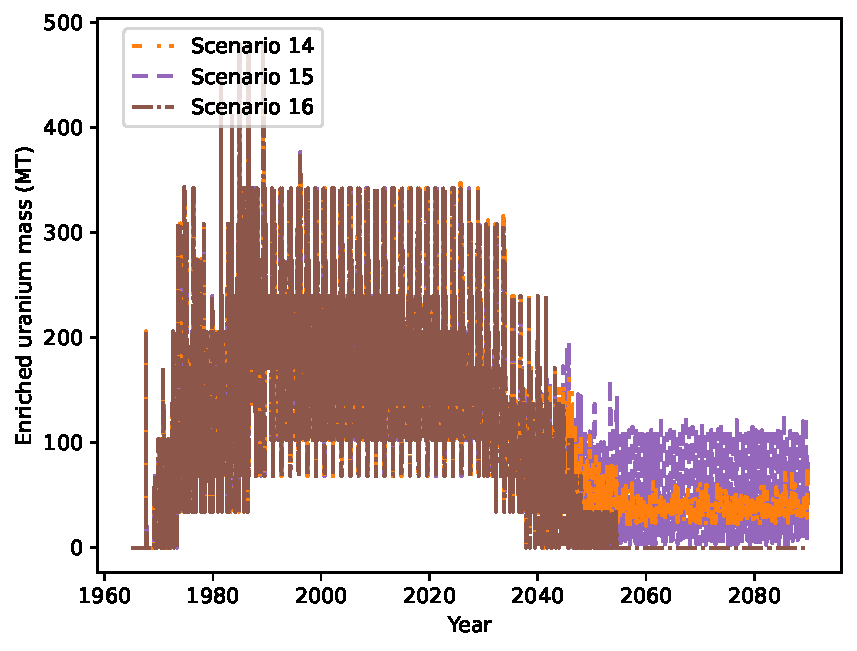
\includegraphics[width=\textwidth]{nogrowth_recycle_total_fuel.pdf}
        \caption{Monthly mass sent to all reactors 
        between 1965-2090.}
        \label{fig:nogrowth_recycle_all_uranium}
    \end{subfigure}
    \hfill
    \begin{subfigure}[b]{0.45\textwidth}
        \centering
        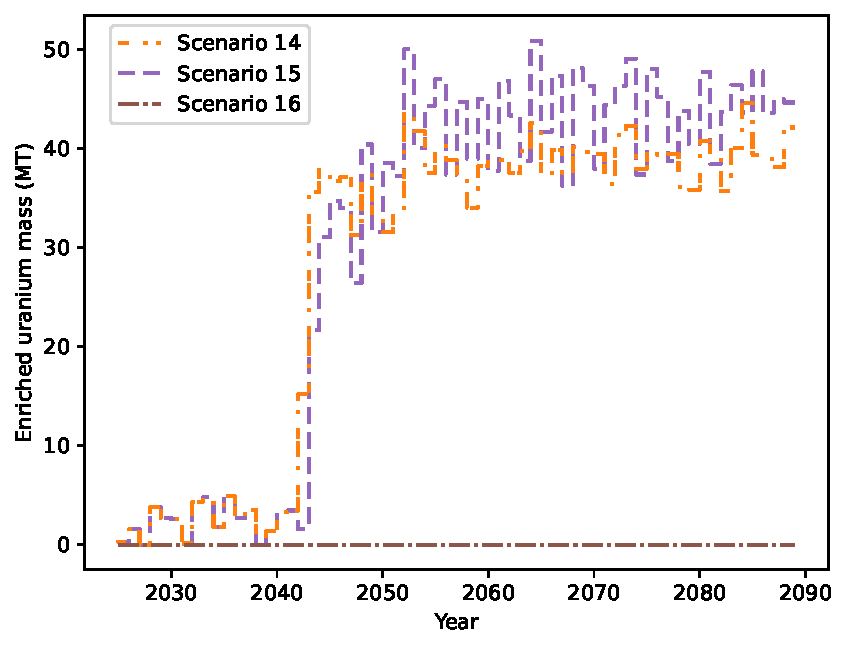
\includegraphics[width=\textwidth]{nogrowth_recycle_Uaverages.pdf}
        \caption{Annual average mass sent to 
        advanced reactors between 2025-2090.}
        \label{fig:nogrowth_recycle_AR_uranium}
    \end{subfigure}
    \begin{subfigure}[b]{0.45\textwidth}
        \centering
        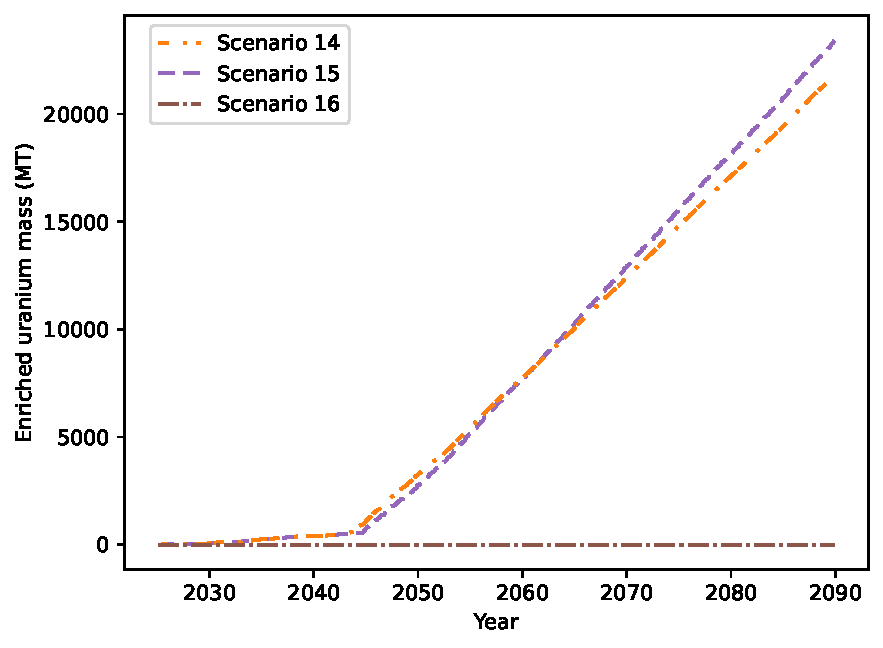
\includegraphics[width=\textwidth]{nogrowth_recycle_Ucumulative.pdf}
        \caption{Cumulative mass sent to advanced reactors between 2025-2090.}
        \label{fig:nogrowth_recycle_uranium_cumulative}
    \end{subfigure}
       \caption{Mass of enriched uranium required by reactors
        in Scenarios 14-16.}
       \label{fig:nogrowth_recycle_uranium}
\end{figure}

Scenario 16 does not require any uranium-based fuel to support the 
advanced reactors. This result stems from a few key differences between 
Scenario 16 and the other no growth closed fuel cycle scenarios. The 
first difference is that all of the advanced 
reactors in Scenario 16 can accept reprocessed fuel, while the \glspl{MMR} 
in Scenarios 14 and 15 will only accept \gls{UOX}. This modeling 
decision for the \gls{MMR} means that any fuel cycle that 
deploys the \gls{MMR} will always require some amount of uranium-based 
fuel. Therefore, the lack of \gls{MMR} deployment in Scenario 16 allows 
the possibility for this scenario to not require enriched uranium. 
The second difference is the reprocessing scheme.  
In Scenario 16, the spent fuel can be reprocessed an infinite number 
of times while in Scenarios 14 and 15 the spent uranium-based fuel can 
only be reprocessed once and the plutonium-based fuel can not be 
reprocessed. This difference is inherent to the type of fuel cycle 
(limited vs. continuous recycle), and increases the amount of 
\gls{SNF} available for reprocessing. Additionally, the reprocessing 
step in Scenario 16 removes the uranium, neptunium, plutonium, 
and americium from the spent fuel, compared with only plutonium 
being separated out in Scenarios 14 and 15. Allowing more material 
to be separated out of the \gls{SNF} in Scenario 16 leads to more 
separated actinide material to create the plutonium-based fuel. 

Table \ref{tab:s14-16_uranium} reports the average enriched uranium mass, 
average \gls{HALEU} mass, maximum enriched uranium mass, and cumulative 
enriched uranium mass required in Scenarios 14-16. Scenario 14 requires 
less enriched uranium than Scenario 7, despite having the same 
advanced reactor deployment schedule, because of the change in the 
fuel cycle. By reprocessing spent fuel, the average \gls{HALEU} 
mass required drops by 21.3\%. A similar decrease in cumulative 
\gls{HALEU} needs is seen in Scenario 15. However, the removal of 
\gls{TRISO} reprocessing results in a smaller decrease (15.1\%
decrease). By reprocessing the \gls{TRISO}-based fuels in 
Scenario 14, this scenario needs 6.35\% less enriched uranium, 
cumulative, than Scenario 15. 

\begin{table}[h!]
    \centering 
    \caption{Metrics for enriched uranium required to fuel reactors 
    in Scenarios 14-16.}
    \label{tab:s14-16_uranium}
    \begin{tabular}{c c c c c}
        \hline 
        Scenario & Average (MT/month) & HALEU Average (MT/month) 
        & Maximum (MT) & Cumulative (MT) \\
        \hline 
        14 & 28.01 & 27.16 & 87.01 & 21,920 \\
        15 & 30.05 & 29.20 & 143.8 & 23,407\\
        16 & 0 & 0 & 0 & 0\\
        \hline
        
    \end{tabular}
\end{table}

Scenarios 14, 15, and 16 require a cumulative enriched uranium 
mass of 3,162, 2,667, and 0 MT, respectively, by 2050. These values 
are smaller than the needs of the once-through fuel cycles 
(Table \ref{tab:nogrowth_haleu}) and the estimated 5,350 MT from 
Dixon et al. \cite{dixon_estimated_2022}. The closed fuel cycle 
scenarios require less \gls{HALEU} than the once-through 
fuel cycles because of the inclusion of reprocessing and use 
of plutonium-based fuel in the advanced reactors. 

In addition to the enriched uranium, the advanced 
reactors receive heavy metals for the plutonium-based 
fuels. Figure 
\ref{fig:nogrowth_recycle_mox} shows that Scenario 16 requires more 
plutonium-based fuel than the other scenarios. This result is consistent 
with the reactors in Scenarios 16 not receiving any enriched 
uranium. Scenario 14 uses the next largest mass of heavy metals for 
plutonium-based fuel, followed by Scenario 15. However, the 
magnitude of the masses between Scenario 16 and Scenarios 14-15 is 
different. 

\begin{figure}[h!]
    \centering
    \begin{subfigure}[b]{0.45\textwidth}
        \centering
        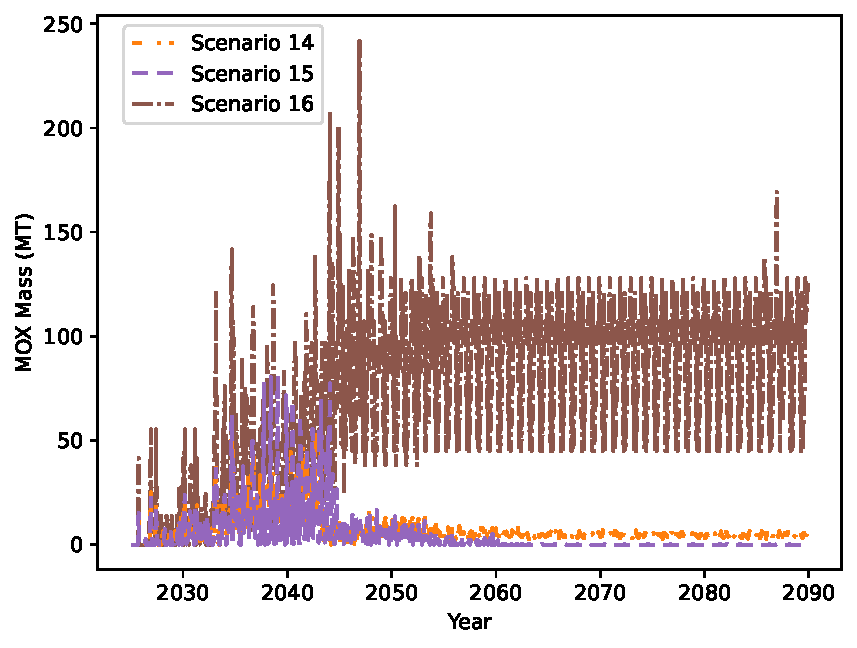
\includegraphics[width=\textwidth]{nogrowth_recycle_MOX.pdf}
        \caption{Monthly masses sent to 
        advanced reactors between 2025-2090.}
        \label{fig:nogrowth_recycle_AR_mox}
    \end{subfigure}
    \hfill
    \begin{subfigure}[b]{0.45\textwidth}
        \centering
        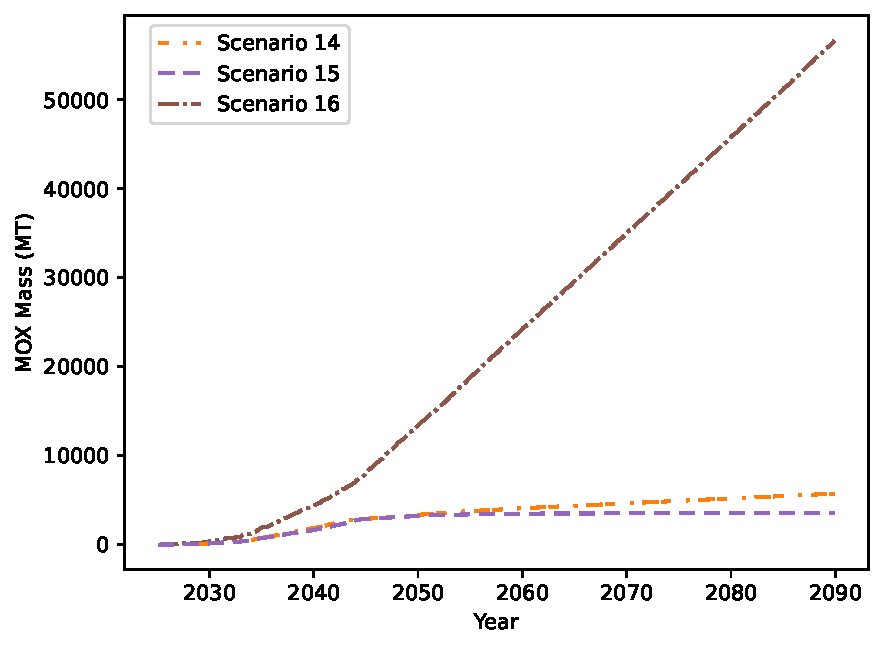
\includegraphics[width=\textwidth]{nogrowth_recycle_MOXcumulative.pdf}
        \caption{Cumulative mass 
        sent to advanced reactors between 2025-2090.}
        \label{fig:nogrowth_recycle_mox_cumulative}
    \end{subfigure}
       \caption{Mass of plutonium-based fuel required by reactors
        in Scenarios 14-16.}
       \label{fig:nogrowth_recycle_mox}
\end{figure}

As Table \ref{tab:s14-16_mox} reports, the average and cumulative 
masses of plutonium-based fuel heavy metals in Scenario 16 and 
Scenario 14-15 differ by an oder of magnitude. This large difference 
is a result of the different reprocessing schemes, as previously 
described. 
Scenario 16 needs a monthly average 
of plutonium-based fuel heavy metal that is more than the maximum mass 
needed in Scenario 14. More heavy metal for plutonium-based fuel
is sent to advanced reactor in Scenario 14 than  
in Scenario 15 because of the greater availability of 
plutonium-based fuel because of the reprocessing of 
\gls{TRISO}-based fuel in Scenario 14. The heavy metals for plutonium fuels 
in Scenarios 14 and 15 show a decrease in 2043, corresponding 
to the increase in enriched uranium sent to reactors in these 
scenarios. After the initial stock of plutonium-based fuel 
from \gls{LWR} spent fuel is used in Scenarios 14 and 15, these 
scenarios use an 
average of 5.26 MT/month and 1.49 MT/month, respectively. These 
values are both smaller than the average values reported 
in Table \ref{tab:s14-16_mox}, highlighting the importance 
of a stockpile of plutonium-based fuel from \gls{LWR} spent 
fuel in providing plutonium-based fuel for advanced reactors in these fuel 
cycles. 

\begin{table}[h!]
    \centering 
    \caption{Metrics for plutonium-based fuels required to fuel reactors 
    in Scenarios 14-16.}
    \label{tab:s14-16_mox}
    \begin{tabular}{c c c c}
        \hline 
        Scenario & Average (MT/month) & Maximum (MT) & Cumulative (MT) \\
        \hline 
        14 & 7.351 & 53.81 & 5,727 \\
        15 & 4.506 & 81.59 & 3,510 \\
        16 & 72.70 & 241.9 & 56,630 \\
        \hline
        
    \end{tabular}
\end{table}

When comparing the total cumulative mass of heavy metal (enriched 
uranium and heavy metal in plutonium-based fuel) required by each scenario,
Scenario 16 needs the most material of these three scenarios. This 
result stems from the different discharge burnups of the reactors. The 
\gls{SFR} has a burnup of 87.51 MWd/kg HM and the Xe-100 (the reactor that 
meets most of the demand in Scenarios 14 and 15) has a burnup of 168 MWd/kg U. 
The Xe-100 gets more energy out of each unit mass of fuel, which leads to 
Scenarios 14 and 15 requiring less fuel than Scenario 16. Scenario 16 is most 
similar to Scenario 2 in the amount of heavy metals required, because
the \gls{SFR} and \gls{MMR} have similar discharge burnups (87.51 MWd/kg 
compared with 82.6 MWd/kg).

\subsubsection{Natural uranium}
Figure \ref{fig:nogrowth_recycle_feed} shows 
the natural uranium required as feed uranium to produce enriched 
uranium fuel for advanced reactors in Scenarios 14-16.  
Scenario 15 requires 
the most feed uranium, followed by Scenarios 14 and 16. This pattern follows 
with the enriched uranium mass in each scenario, because the enriched 
uranium mass dictates the amount of feed uranium needed.
Scenario 15 requires the 
most feed mass because less \gls{SNF} is available for reprocessing, 
leading to more 
enriched uranium required. Scenario 
16 does not requires any feed uranium because it does not require any 
enriched uranium. 

\begin{figure}[h!]
    \centering
    \begin{subfigure}[b]{0.45\textwidth}
        \centering
        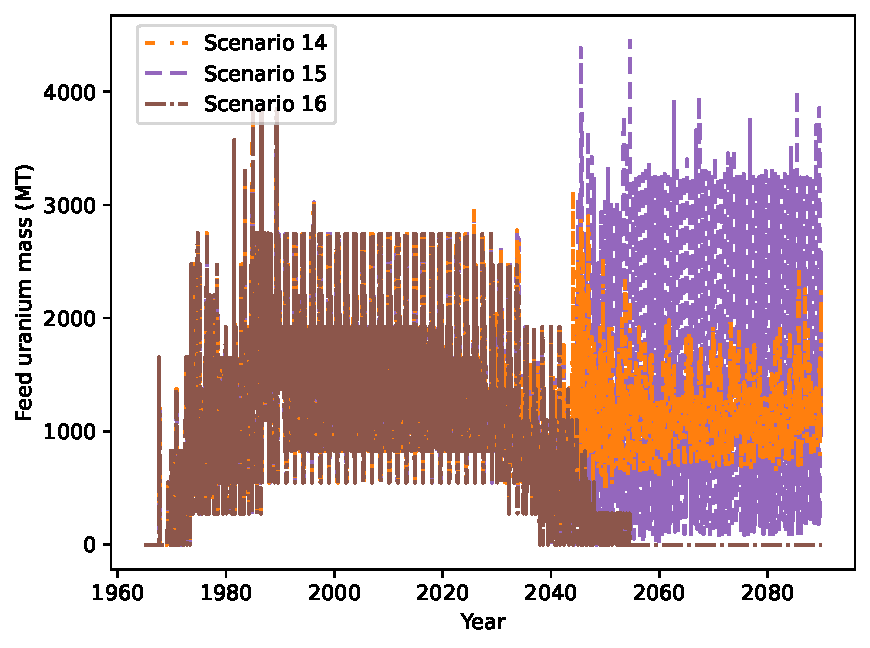
\includegraphics[width=\textwidth]{nogrowth_recycle_feed.pdf}
        \caption{Monthly mass 
        to support all reactors between 1965-2090.}
        \label{fig:nogrowth_recycle_all_feed}
    \end{subfigure}
    \hfill
    \begin{subfigure}[b]{0.45\textwidth}
        \centering
        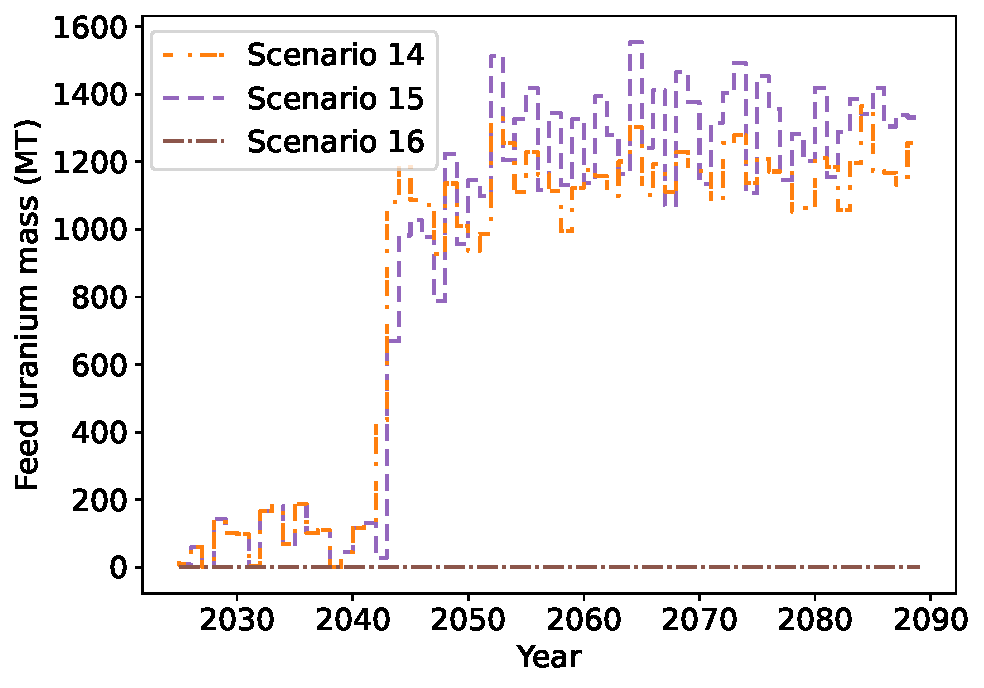
\includegraphics[width=\textwidth]{nogrowth_recycle_feed_average.pdf}
        \caption{Annual average  mass 
        to support advanced reactors between 2025-2090.}
        \label{fig:nogrowth_recycle_AR_feed}
    \end{subfigure}
    \begin{subfigure}[b]{0.45\textwidth}
        \centering
        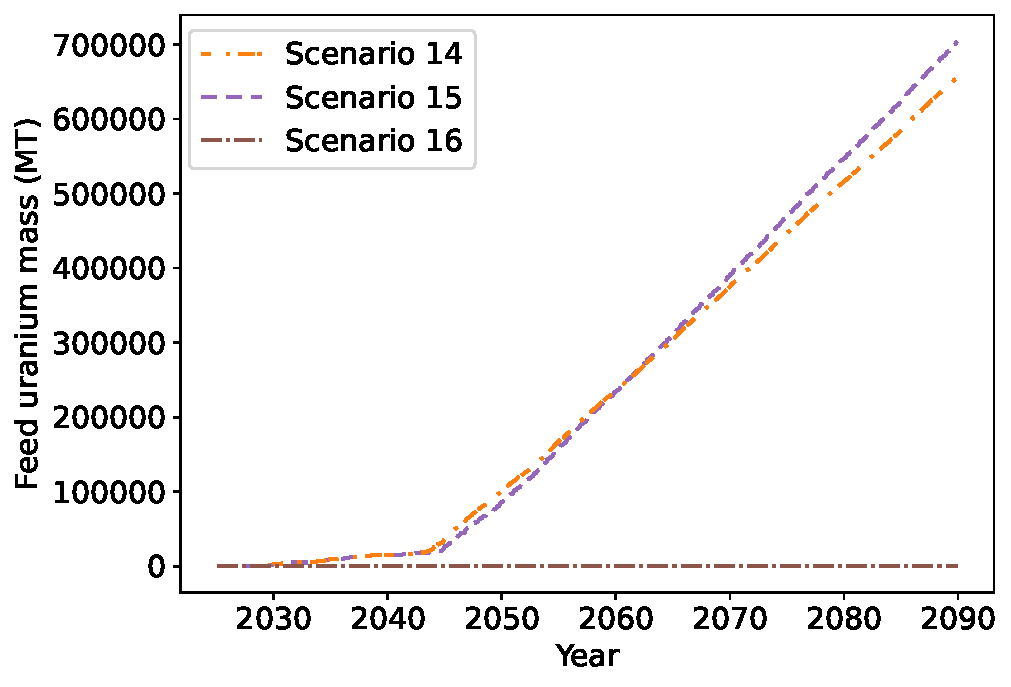
\includegraphics[width=\textwidth]{nogrowth_recycle_feed_cumulative.pdf}
        \caption{Cumulative mass to support advanced reactors between 2025-2090.}
        \label{fig:nogrowth_recycle_feed_cumulative}
    \end{subfigure}
       \caption{Mass of feed uranium required by reactors
        in Scenarios 14-16.}
       \label{fig:nogrowth_recycle_feed}
\end{figure}

Table \ref{tab:s14-16_feed} reports the metrics for the feed uranium 
required in Scenarios 14-16. The cumulative feed uranium needed in 
Scenarios 14 and 15 are both less than the cumulative feed uranium 
needed in Scenario 7. The decrease in feed uranium needed demonstrates 
how using a closed fuel cycle can reduce the feed uranium needs in 
addition to reducing the fuel mass needs. 

\begin{table}[h!]
    \centering 
    \caption{Metrics for feed uranium required to produce 
    uranium-based fuels in in Scenarios 14-16.}
    \label{tab:s14-16_feed}
    \begin{tabular}{c c c c c}
        \hline 
        Scenario & Average (MT/month) & HALEU Average (MT/month) &
        Maximum (MT) & Cumulative (MT) \\
        \hline 
        14 & 842.9 & 836.4 & 2,628 & 656,582 \\
        15 & 903.9 & 897.4 & 4,450 & 704,106\\
        16 & 0 & 0 & 0 & 0\\
        \hline
        
    \end{tabular}
\end{table}

Next, Figure \ref{fig:nogrowth_recycle_natu} shows the natural 
uranium required for the plutonium-based fuels in Scenarios 14-16. 
These results follow the same pattern as the heavy metal for 
plutonium-based fuels in these scenarios. However, the natural 
uranium mass is less than the total heavy metal mass, because the 
uranium is only a part of the total heavy metal mass. Scenario 16 requires 
the most natural uranium because the reactors in this scenario 
only receive the U/TRU fuel. Scenario 15 requires the least 
natural uranium, because this scenario results in the least 
plutonium-based fuel.

\begin{figure}[h!]
    \centering
    \begin{subfigure}[b]{0.45\textwidth}
        \centering
        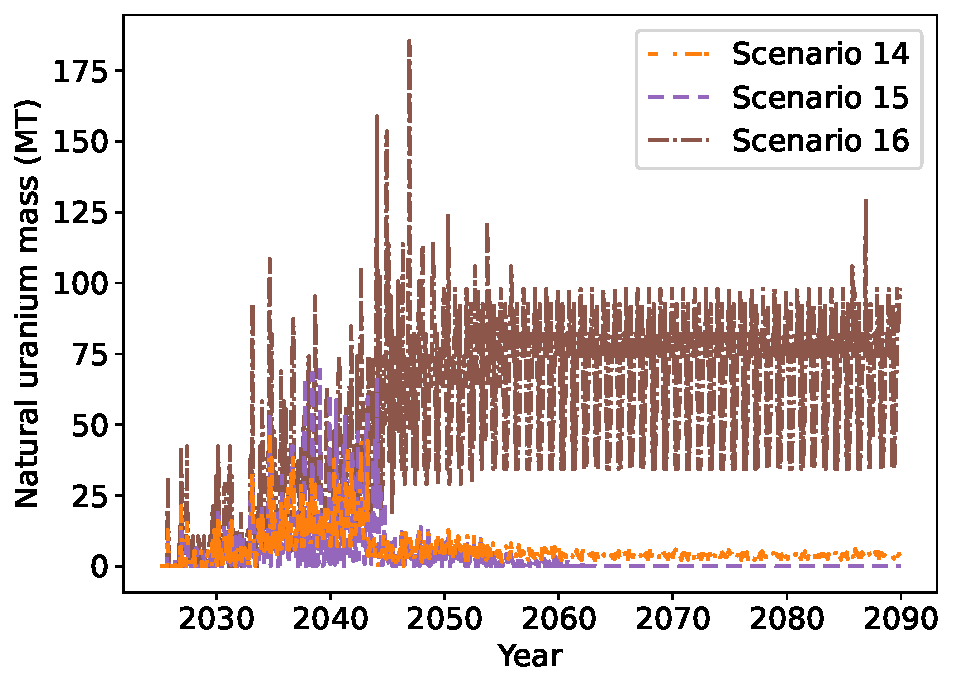
\includegraphics[width=\textwidth]{nogrowth_recycle_natU.pdf}
        \caption{Monthly mass to support
        advanced reactors between 2025-2090.}
        \label{fig:nogrowth_recycle_AR_natu}
    \end{subfigure}
    \hfill
    \begin{subfigure}[b]{0.45\textwidth}
        \centering
        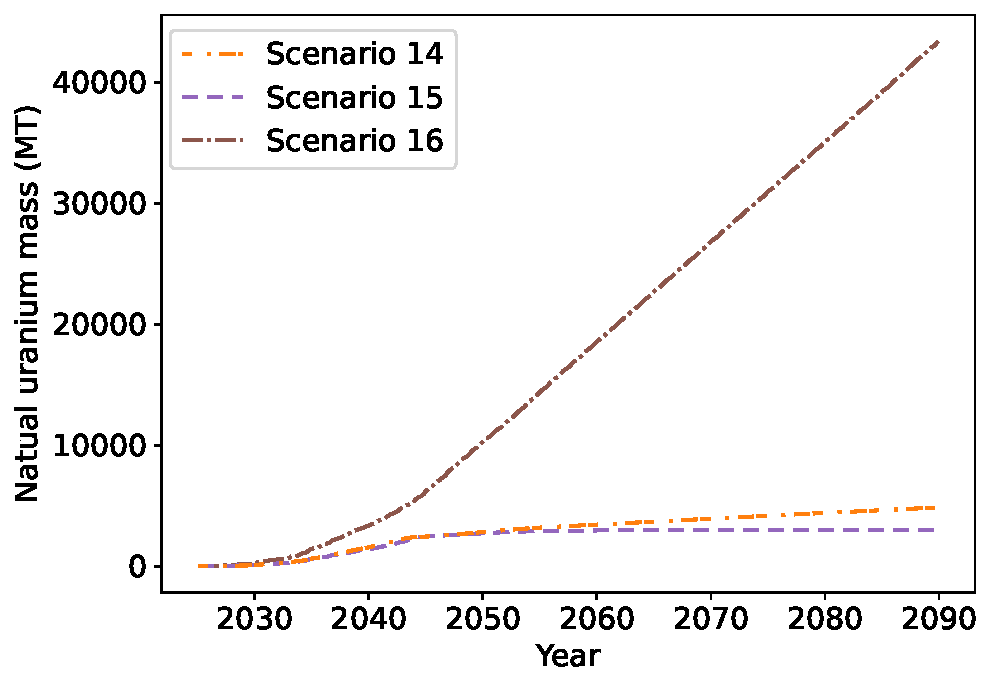
\includegraphics[width=\textwidth]{nogrowth_recycle_natU_cumulative.pdf}
        \caption{Cumulative mass to support advanced reactors between 2025-2090.}
        \label{fig:nogrowth_recycle_natu_cumulative}
    \end{subfigure}
       \caption{Mass of natural uranium for plutonium-based fuel required 
       by reactors
        in Scenarios 14-16.}
       \label{fig:nogrowth_recycle_natu}
\end{figure}

Table \ref{tab:s14-16_natU} reports the metrics fo the natural uranium 
required for Scenarios 14-16. The metrics for Scenario 16 are one order 
of magnitude greater than the metrics for Scenarios 14-15, the same as 
the metrics of the plutonium-based fuel heavy metal. 
The cumulative natural uranium mass 
needed by Scenario 16 is more than one order of magnitude smaller than 
the cumulative feed uranium masses in Scenarios 14 and 15, because of the 
difference in process losses in each use of natural uranium. Using natural 
uranium as fill material in plutonium-based fuel has relatively small 
process losses because the material is used in its direct form. However, 
using natural uranium as feed for enrichment has large material losses 
(referred to as the tails material stream)
because of the low enrichment of natural uranium (0.711\%). Based on 
Eq. \ref{eq:enrichment}, the process losses increase with increased 
product mass demand and with increased product assay. The different 
masses of natural uranium for use in plutonium-based fuel and 
for enrichment suggests that fuel cycle that maximizes 
the amount of plutonium-based fuel and minimizes the amount of 
enriched uranium required helps to minimize natural uranium requirements. 

\begin{table}[h!]
    \centering 
    \caption{Metrics for natural uranium required to produce 
    plutonium-based fuels in Scenarios 14-16.}
    \label{tab:s14-16_natU}
    \begin{tabular}{c c c c}
        \hline 
        Scenario & Average (MT/month) & Maximum (MT) & Cumulative (MT) \\
        \hline 
        14 & 6.256 & 45.80 & 4,874 \\
        15 & 3.835 & 69.44 & 2,987 \\
        16 & 55.68 & 185.3 & 43,372 \\
        \hline
        
    \end{tabular}
\end{table}

\subsection{1\% growth scenarios}
This section presents the results of the uranium resources required 
in the 1\% growth, closed fuel cycle scenarios (Scenarios 17-19). 
We divide these results into the fuel masses (enriched uranium 
and heavy metals in plutonium-based fuel) and the natural 
uranium masses (feed uranium and natural uranium to produce 
plutonium-based fuels).

\subsubsection{Fuel masses}
The first fuel mass considered is the enriched uranium mass, 
shown in Figure \ref{fig:1percent_recycle_uranium}. These results 
show the same pattern as this metric for the no growth scenarios:
Scenario 18 requires the most enriched uranium and Scenario 19 
does not require any enriched uranium. In Scenarios 17 and 18 the 
increase in enriched uranium need occurs closer to 2040 and is a 
more gradual increase than the observed increase in Scenarios 14-15. 
These results stem from differences in the growth in energy 
demand, and subsequent differences in reactor deployment, leading to the stockpile 
of plutonium-based fuel from \gls{LWR} \gls{SNF} to be used up sooner. 
The differences in energy demand and reactor deployment lead to different 
proportions of the advanced reactors, specifically the artificially
inflated number of \gls{MMR} deployed in these scenarios. These differences 
then leads to the more gradual increase in the enriched uranium needs
because of the slow increase in the number of \glspl{MMR} deployed.

\begin{figure}[h!]
    \centering
    \begin{subfigure}[b]{0.45\textwidth}
        \centering
        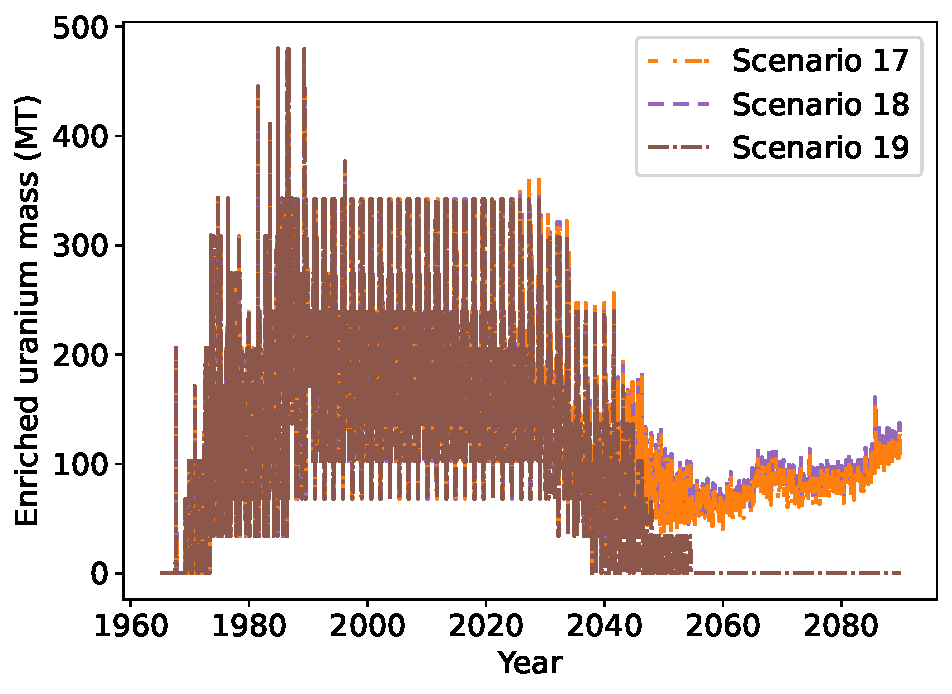
\includegraphics[width=\textwidth]{1percent_recycle_total_fuel.pdf}
        \caption{Monthly mass sent to all reactors 
        between 1965-2090.}
        \label{fig:1percent_recycle_all_uranium}
    \end{subfigure}
    \hfill
    \begin{subfigure}[b]{0.45\textwidth}
        \centering
        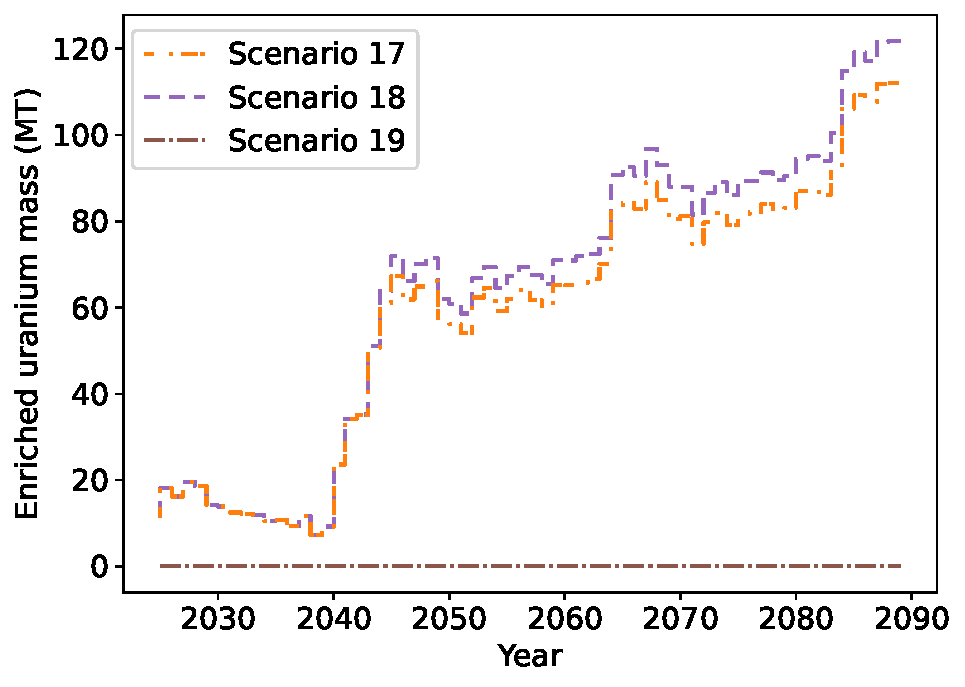
\includegraphics[width=\textwidth]{1percent_recycle_Uaverages.pdf}
        \caption{Annual average mass sent to 
        advanced reactors between 2025-2090.}
        \label{fig:1percent_recycle_AR_uranium}
    \end{subfigure}
    \begin{subfigure}[b]{0.45\textwidth}
        \centering
        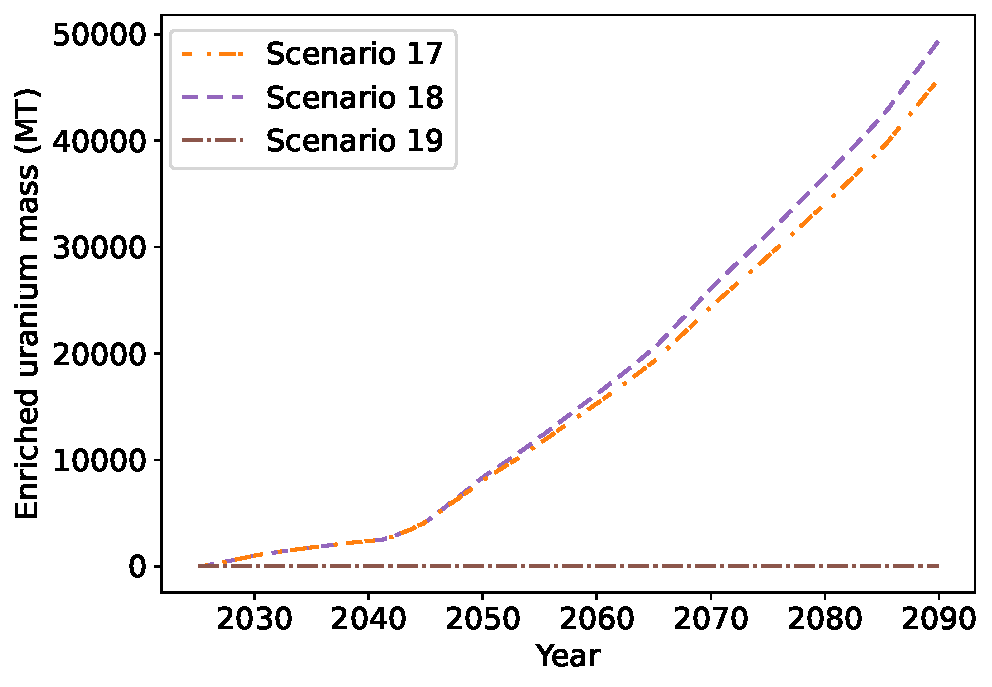
\includegraphics[width=\textwidth]{1percent_recycle_Ucumulative.pdf}
        \caption{Cumulative mass sent to advanced reactors between 2025-2090.}
        \label{fig:1percent_recycle_uranium_cumulative}
    \end{subfigure}
       \caption{Mass of enriched uranium required by reactors
        in Scenarios 17-19.}
       \label{fig:1percent_recycle_uranium}
\end{figure}

Table \ref{tab:s17-19_enrichedU} reports the metrics for the enriched 
uranium masses for Scenarios 17-19. The cumulative enriched 
uranium in Scenarios 17 and 18 are less than the cumulative 
enriched uranium required by Scenario 13. However, the cumulative 
mass for Scenario 18 is larger than the cumulative in Scenario 
9. These results highlight how reprocessing can reduce enriched 
uranium needs, but the reactors deployed and their fuel usage 
is still an important factor in how much enriched uranium is 
needed. 

\begin{table}[h!]
    \centering 
    \caption{Metrics of enriched uranium fuel between 2025-2090 in Scenarios 
    17-19.}
    \label{tab:s17-19_enrichedU}
    \begin{tabular}{c c c c c}
        \hline 
        Scenario & Average (MT/month) & Average HALEU (MT/month) &  
        Maximum (MT) & Cumulative (MT) \\
        \hline
        17 & 58.72 & 52.81 & 152.2 & 45,742\\
        18 & 63.32 & 57.42 & 160.9 & 49,329\\
        19 & 0 & 0 & 0 & 0\\
        \hline
    \end{tabular}
\end{table}

Next is the mass of plutonium-based fuels sent to the advanced reactors 
in Scenarios 17-19, shown in Figure \ref{fig:1percent_recycle_mox}.
Similar to the patterns of the no growth scenarios, Scenario 19 
requires the most 
plutonium-based fuel of the three scenarios and Scenario 17 
requires more than Scenario 18. Scenarios 17 and 18 show the 
initial stockpile of plutonium-based fuel from \gls{LWR} \gls{SNF} that 
gets used by 2040. The plutonium-based fuel mass in Scenario 18 
drops to near zero after 2060, because all of the spent fuel from 
the \glspl{LWR} has been processed and used to create plutonium-based 
fuel, 
and there are so few VOYGRs (the only advanced reactor spent fuel 
reprocessed in this scenario) to produce more separated plutonium 
and more \gls{MOX}. The differences in the plutonium-based fuel 
heavy metal masses in these three scenarios is primarily 
a function of the reprocessing scheme of each scenario. 

\begin{figure}[h!]
    \centering
    \begin{subfigure}[b]{0.45\textwidth}
        \centering
        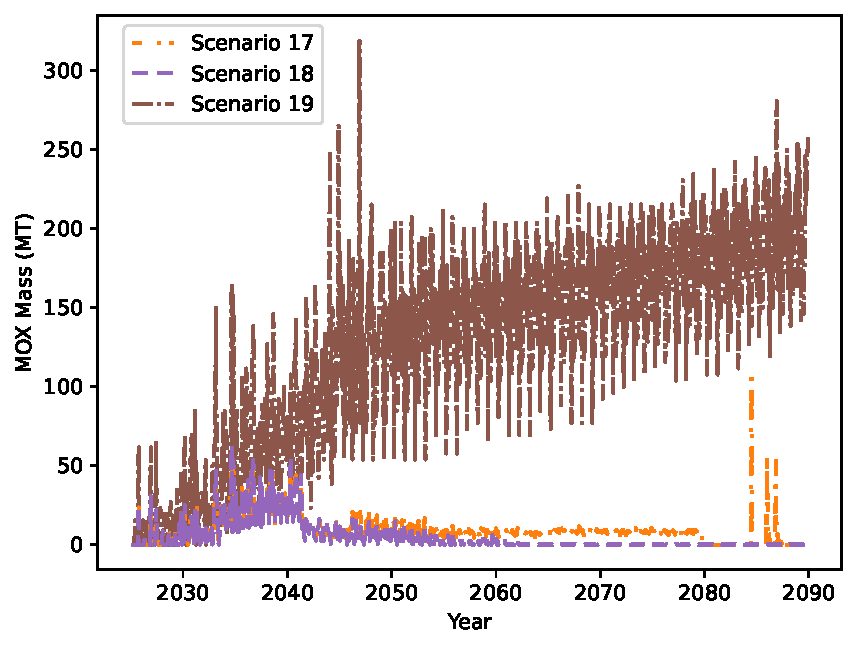
\includegraphics[width=\textwidth]{1percent_recycle_MOX.pdf}
        \caption{Monthly mass sent to all reactors 
        between 1965-2090.}
        \label{fig:1percent_recycle_AR_mox}
    \end{subfigure}
    \hfill
    \begin{subfigure}[b]{0.45\textwidth}
        \centering
        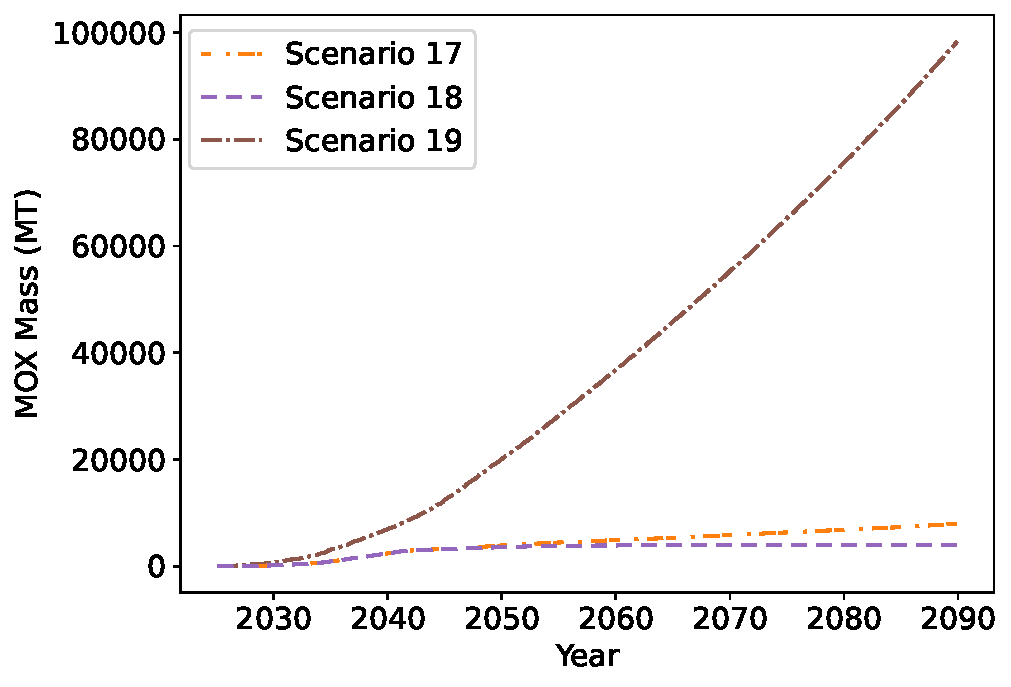
\includegraphics[width=\textwidth]{1percent_recycle_MOXcumulative.pdf}
        \caption{Cumulative mass  
        sent to advanced reactors between 2025-2090.}
        \label{fig:1percent_recycle_mox_cumulative}
    \end{subfigure}
       \caption{Masses of heavy metal in plutonium-based fuel 
        sent to advanced reactors
        in Scenarios 17-19.}
       \label{fig:1percent_recycle_mox}
\end{figure}

Table \ref{tab:s17-19_mox} reports the metrics for the
heavy metals in plutonium-based 
fuels required in Scenarios 17-19. Scenario 19 uses the largest 
heavy metal mass, followed by Scenario 17, then 18. 
Scenario 19 requires more total heavy metal (in enriched 
uranium and plutonium-based fuels) than Scenarios 
17 and 18, as well as Scenarios 9, 10, 12, and 13. Scenario 19 
uses the most similar cumulative mass of heavy metal as Scenario 8, 
because the \gls{MMR} and \gls{SFR} have the most similar burnups 
of the advanced reactors considered. However, Scenario 19 requires 
less heavy metal than Scenario 8 because the \gls{SFR} has a higher 
burnup than the \gls{MMR}. These results emphasize how the 
the reactors deployed play an important role in determining how 
much fuel is required for a fuel cycle.  

\begin{table}[h!]
    \centering 
    \caption{Metrics of plutonium-based fuel between 2025-2090 in Scenarios 
    17-19.}
    \label{tab:s17-19_mox}
    \begin{tabular}{c c c c}
        \hline 
        Scenario & Average (MT/month) & Maximum (MT) & Cumulative (MT) \\
        \hline
        17 & 10.25 & 62.56 & 7,987\\
        18 & 5.109 & 62.56 & 3,979\\
        19 & 126.2 & 318.7 & 98,323\\
        \hline
    \end{tabular}
\end{table}

\subsubsection{Natural uranium}
The next two metrics are related to the natural uranium requirements of 
Scenarios 17-19. The first of these two metrics is the 
natural uranium needed as feed material for enrichment, shown in 
Figure \ref{fig:1percent_recycle_feed}. The feed uranium masses follow with 
the enriched uranium masses in these scenarios, because of 
the relationship between these two metrics. Scenario 18 requires 
the most feed uranium, and Scenario 19 requires no feed uranium. 
There is increased demand for feed uranium with time in Scenarios 17 
and 18, resulting from the increased energy demand 
and the increased demand of uranium-based fuel in the scenarios.  

\begin{figure}[h!]
    \centering
    \begin{subfigure}[b]{0.45\textwidth}
        \centering
        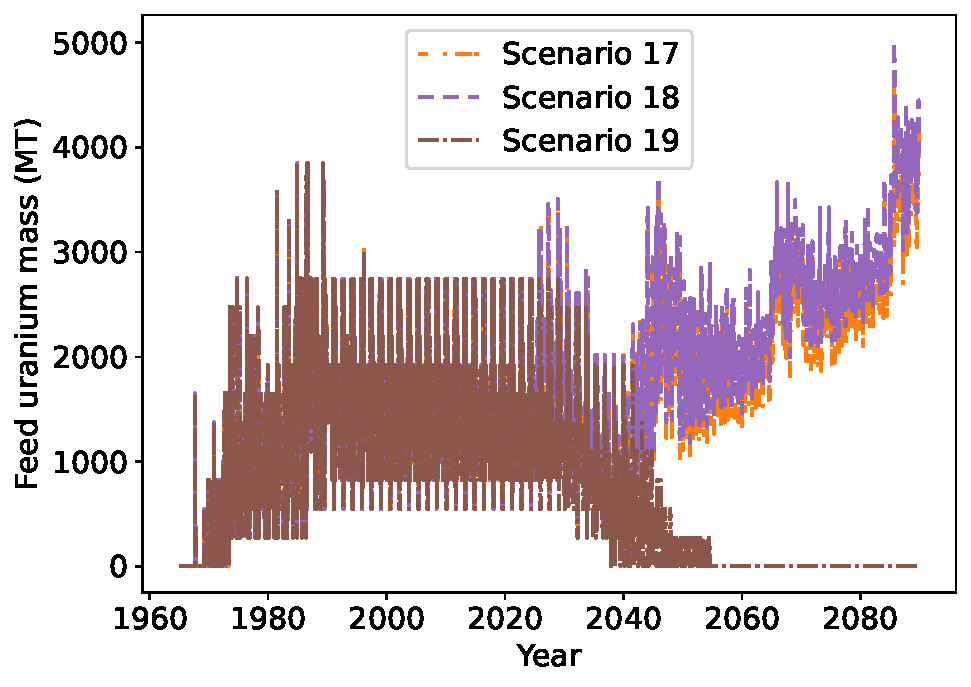
\includegraphics[width=\textwidth]{1percent_recycle_feed.pdf}
        \caption{Monthly mass to support all reactors 
        between 1965-2090.}
        \label{fig:1percent_recycle_all_feed}
    \end{subfigure}
    \hfill
    \begin{subfigure}[b]{0.45\textwidth}
        \centering
        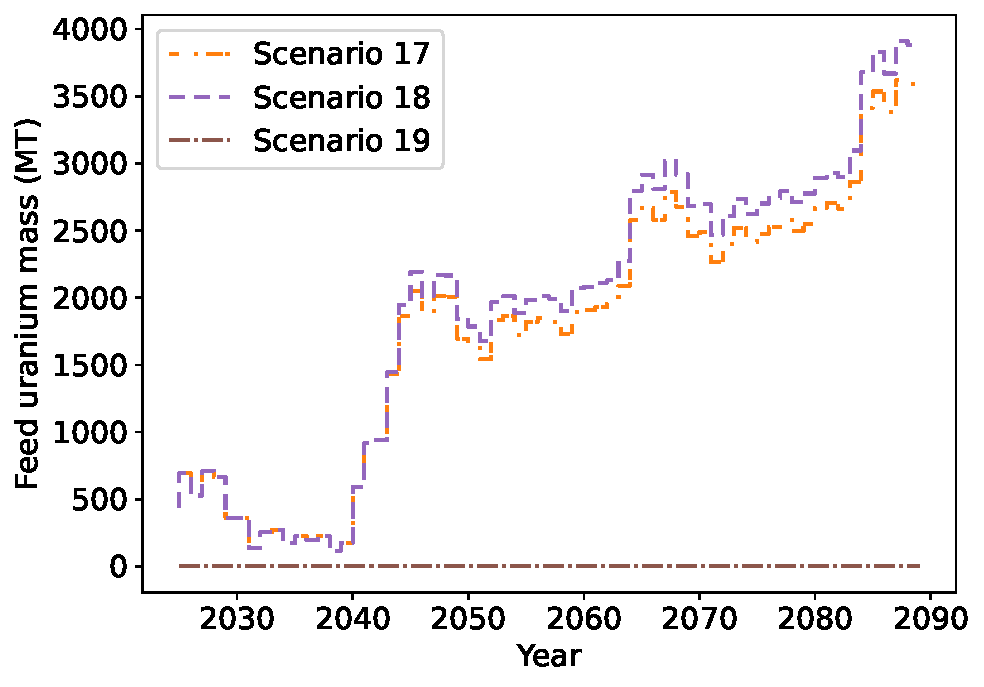
\includegraphics[width=\textwidth]{1percent_recycle_feed_average.pdf}
        \caption{Annual average mass to support
        advanced reactors between 2025-2090.}
        \label{fig:1percent_recycle_AR_feed}
    \end{subfigure}
    \begin{subfigure}[b]{0.45\textwidth}
        \centering
        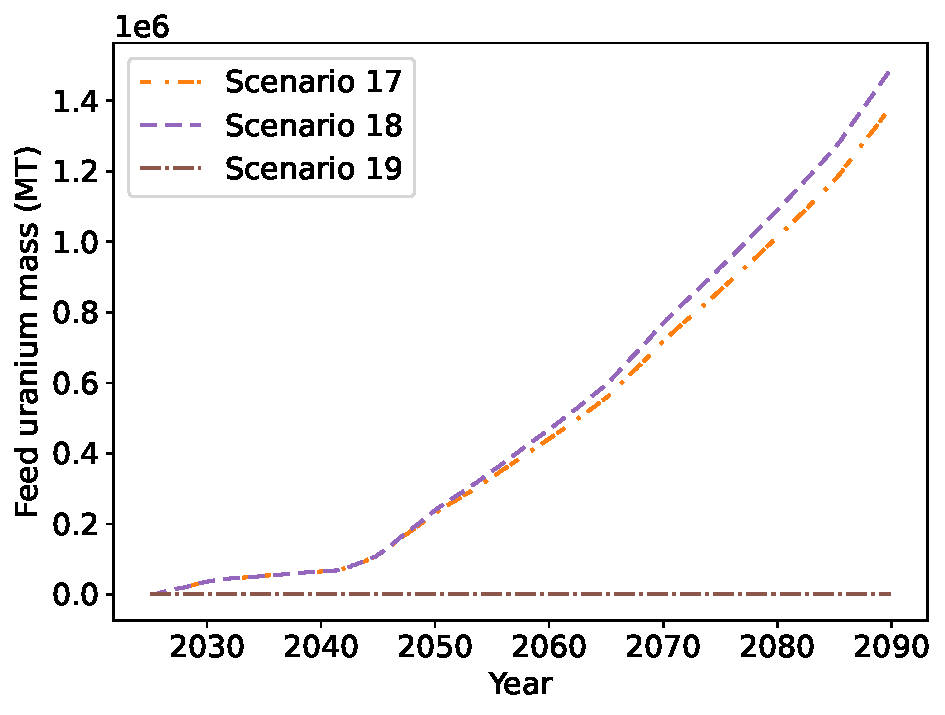
\includegraphics[width=\textwidth]{1percent_recycle_feed_cumulative.pdf}
        \caption{Cumulative mass to support advanced reactors between 2025-2090.}
        \label{fig:1percent_recycle_feed_cumulative}
    \end{subfigure}
       \caption{Masses of feed uranium required by reactors
        in Scenarios 17-19.}
       \label{fig:1percent_recycle_feed}
\end{figure}

Table \ref{tab:s17-19_feed} reports the metrics for the feed uranium in 
Scenarios 17-19. Scenarios 17 and 18 need more feed uranium than 
Scenarios 9 and 12. Scenarios 9 and 12 primarily deploy the Xe-100,
while Scenarios 17 and 18 deploy an inflated number of \glspl{MMR}, 
because of the direct replacement of \glspl{MMR} in the deployment 
scheme. The inflated number of \glspl{MMR} increases the 
feed uranium requirements because the \glspl{MMR} only accept 
\gls{HALEU} fuel in these scenarios, and the \gls{MMR} requires 
more feed uranium per unit energy than the Xe-100. Scenario 19 does not 
require any feed uranium because the \glspl{SFR} in this scenario 
only receive plutonium-based fuel. 

\begin{table}[h!]
    \centering 
    \caption{Metrics of feed uranium to produce enriched uranium 
    between 2025-2090 in Scenarios 17-19.}
    \label{tab:s17-19_feed}
    \begin{tabular}{c c c c c}
        \hline 
        Scenario & Average (MT/month) & HALEU Average (MT/month) & 
        Maximum (MT) & Cumulative (MT) \\
        \hline
        17 & 1,774 & 1,728 & 4,750 & 1,381,600\\
        18 & 1,866 & 1,911 & 5,014 & 1,489,022\\
        19 & 0 & 0 & 0 & 0\\
        \hline
    \end{tabular}
\end{table}

Finally, Figure \ref{fig:1percent_recycle_natU} shows the natural uranium 
required to produce plutonium-based fuels in Scenarios 17-19. Scenario 
19 requires the most natural uranium for plutonium-based fuels, 
followed by Scenario 17, then Scenario 18. The masses of plutonium-based 
fuel drives the demand for this natural uranium, therefore these 
results follow the same patterns seen in Figure \ref{fig:1percent_recycle_mox}.
Scenario 19 requires the most natural uranium for plutonium-based 
fuels because the advanced reactors in this scenario only receive 
plutonium-based fuel, and the \gls{SFR} requires more fuel than 
the Xe-100. 

\begin{figure}[h!]
    \centering
    \begin{subfigure}[b]{0.45\textwidth}
        \centering
        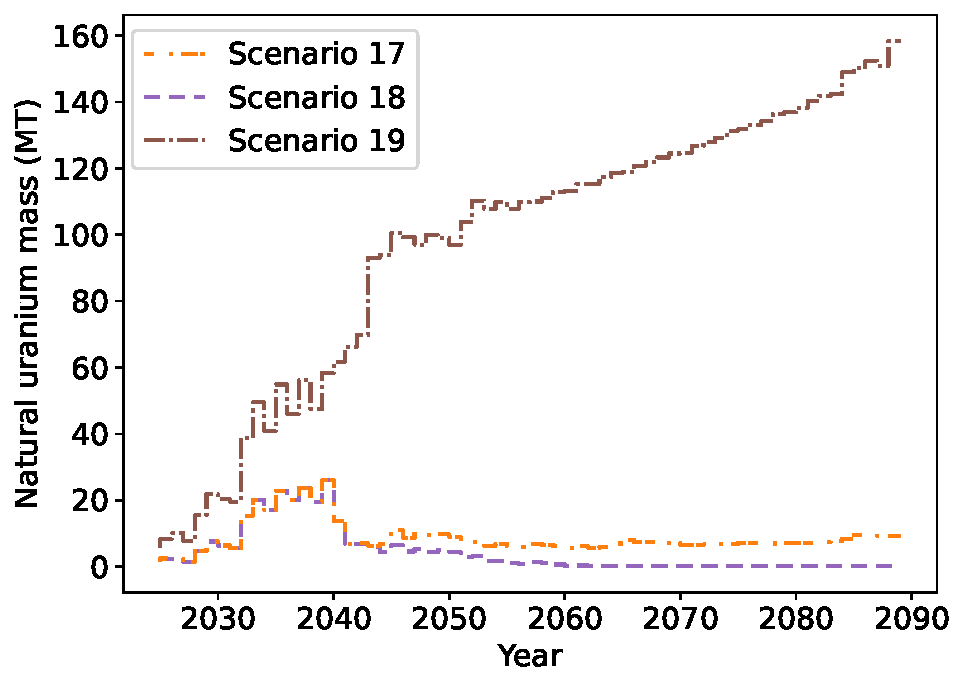
\includegraphics[width=\textwidth]{1percent_recycle_natU.pdf}
        \caption{Monthly mass to support advanced reactors 
        between 1965-2090.}
        \label{fig:1percent_recycle_AR_natu}
    \end{subfigure}
    \hfill
    \begin{subfigure}[b]{0.45\textwidth}
        \centering
        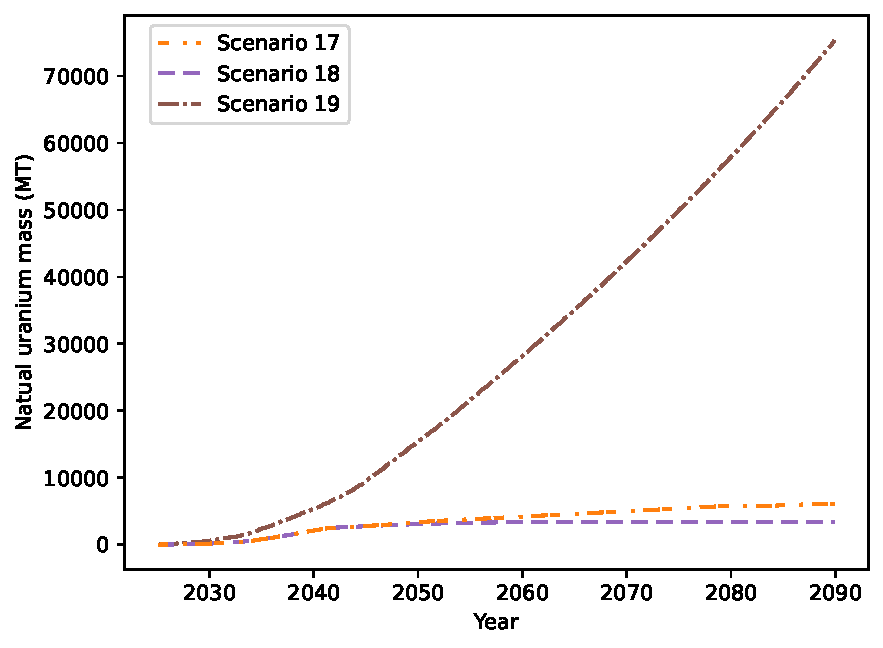
\includegraphics[width=\textwidth]{1percent_recycle_natU_cumulative.pdf}
        \caption{Cumulative mass to support
        advanced reactors between 2025-2090.}
        \label{fig:1percent_recycle_natu_cumulative}
    \end{subfigure}
       \caption{Mass of natural uranium required by reactors in 
       plutonium-based fuels in Scenarios 17-19.}
       \label{fig:1percent_recycle_natU}
\end{figure}

Table \ref{tab:s17-19_natU} reports the metrics for the 
natural uranium for plutonium-based fuels in Scenarios 17-19. 
These metric follow the same pattern observed for the 
no growth scenarios (Scenarios 14-16). Despite Scenario 19 
requiring the most natural uranium for plutonium-based 
fuels, this total is still less than the cumulative feed uranium 
masses required in Scenarios 17 and 18 by almost a factor 
of two. The decreased total 
natural uranium mass in Scenario 19, compared with Scenarios 
17 and 18, is a result of the lack of (or minimal) material loss in 
using natural uranium for plutonium-based fuel, compared with 
the losses from using natural uranium as feed material for 
enrichment. 

\begin{table}[h!]
    \centering 
    \caption{Metrics of natural uranium required to produce 
    plutonium-based fuel between 2025-2090 in Scenarios 
    17-19.}
    \label{tab:s17-19_natU}
    \begin{tabular}{c c c c}
        \hline 
        Scenario & Average (MT/month) & Maximum (MT) & Cumulative (MT) \\
        \hline
        17 & 8.726 & 53.24 & 6,797\\
        18 & 4.348 & 53.24 & 3,387\\
        19 & 96.67 & 244.1 & 75,303\\
        \hline
    \end{tabular}
\end{table}


\section{SWU capacity}
The next category of metrics of interest is the \gls{SWU} capacity required 
to produce the enriched uranium in each of the scenarios. The \gls{SWU} 
capacity has important implications on the enrichment facilities required 
to support these fuel cycles. 

\subsection{No growth scenarios}
Figure \ref{fig:nogrowth_recycle_swu} shows \gls{SWU} capacity required 
in Scenarios 14-16. For Scenarios 14 and 15 the required \gls{SWU} 
capacity for the advanced reactors is relatively small, then increases 
around 2043, corresponding with the increased need for enriched uranium 
for reactors observed in Figure \ref{fig:nogrowth_recycle_uranium}. Scenario 
16 does not require any \gls{SWU} capacity because the advanced reactors 
in this scenario do not receive any enriched uranium. 

\begin{figure}[h!]
    \centering
    \begin{subfigure}[b]{0.45\textwidth}
        \centering
        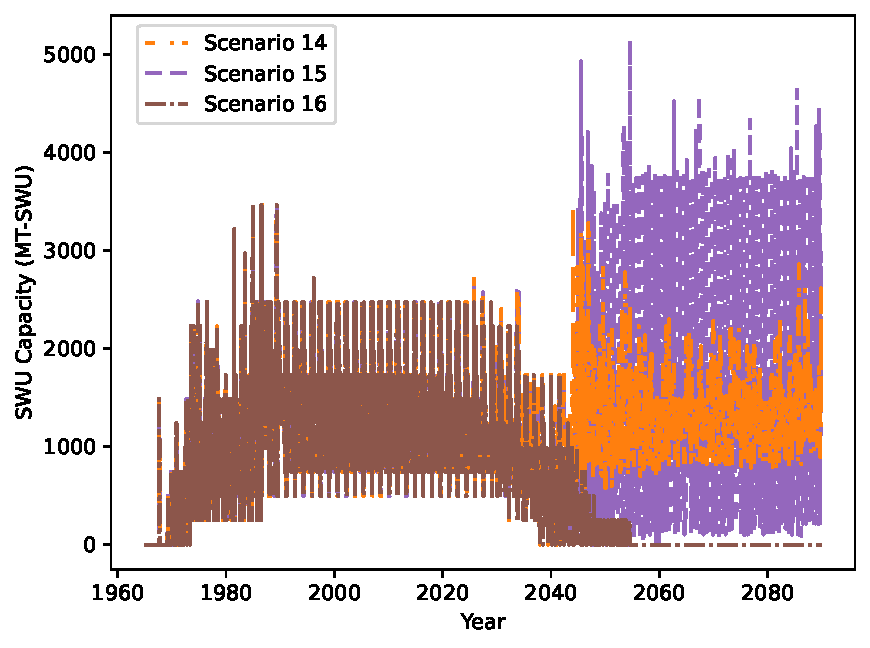
\includegraphics[width=\textwidth]{nogrowth_recycle_swu.pdf}
        \caption{Monthly SWU capacity to support all reactors between 2025-2090.}
        \label{fig:nogrowth_recycle_swu_all}
    \end{subfigure}
    \hfill
    \begin{subfigure}[b]{0.45\textwidth}
        \centering
        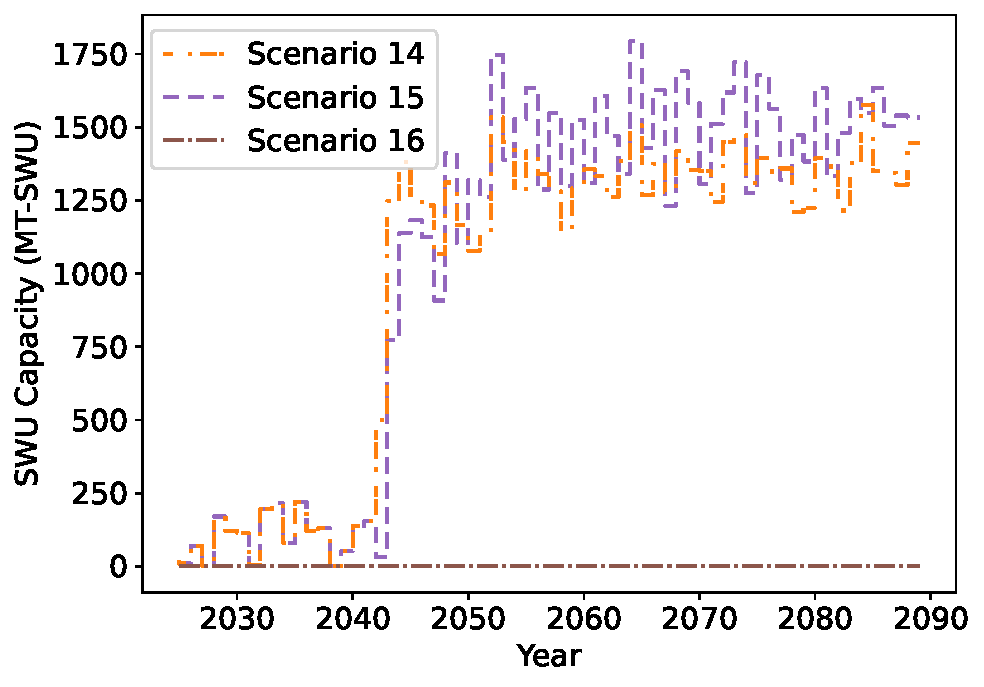
\includegraphics[width=\textwidth]{nogrowth_recycle_AR_swu.pdf}
        \caption{Annual average to support advanced reactors between 2025-2090.}
        \label{fig:nogrowth_recycle_swu_AR}
    \end{subfigure}
       \caption{\gls{SWU} capacity required to support 
       reactors in Scenarios 14-16.}
       \label{fig:nogrowth_recycle_swu}
\end{figure}

Table \ref{tab:s14-16_swu} reports the metrics of required \gls{SWU} 
capacity in Scenarios 14-16. Scenarios 14 and 15 require smaller 
average \gls{SWU} capacities than Scenarios 2-7, and require a 
smaller average \gls{SWU} capacity to produce \gls{HALEU} than 
Scenarios 2, 3, 4, 6, and 7. Scenario 5 requires less \gls{SWU} 
capacity to produce \gls{HALEU} because this scenario 
primarily deploys VOYGRs and requires less \gls{HALEU} than 
any of the no growth scenarios that require \gls{HALEU}. 
The differences in the 
\gls{SWU} capacity needed by these scenarios is a function of 
the reactors deployed and the amount of material available for 
reprocessing. These parameters drive the amount of enriched 
uranium needed in each scenario, which drives the needed 
\gls{SWU} capacity.

\begin{table}[h!]
    \centering 
    \caption{Metrics for \gls{SWU} capacity required to produce 
    enriched uranium in Scenarios 14-16.}
    \label{tab:s14-16_swu}
    \begin{tabular}{c c c c}
        \hline 
        Scenario & Average (MT-SWU/month) & HALEU Average (MT-SWU/month)
         & Maximum (MT-SWU) \\
        \hline 
        14 & 971.6 & 965.9 & 3,032 \\
        15 & 1,042 & 1,036 & 5,142 \\
        16 & 0 & 0 & 0 \\
        \hline
        
    \end{tabular}
\end{table}

The results of these scenarios identify recycling \gls{SNF} as a way 
to reduce the \gls{SWU} capacity required in a fuel cycle. Additionally, 
increasing the amount of \gls{SNF} available for reprocessing further 
reduces the \gls{SWU} capacity required. The lack of needed 
\gls{SWU} capacity in Scenario 16 indicates that developing this 
fuel cycle would not require any new enrichment capacity to be developed 
in the US.  However, the US does not have 
any facilities for reprocessing commercial fuel. Therefore, reprocessing
fuel does not assist in meeting initial \gls{HALEU} demand because 
the US would need to develop new infrastructure to support any 
of these transitions, whether it is enrichment facilities, 
reprocessing facilities, or both.

\subsection{1\% growth scenarios}
Figure \ref{fig:1percent_recycle_swu} shows the \gls{SWU} capacity 
required to enrich uranium in Scenarios 17-19. Similar to the 
feed uranium masses, the mass of enriched uranium drives 
the required \gls{SWU} capacity. Scenario 18 requires the most 
\gls{SWU} capacity, followed by Scenario 17, and Scenario 19 does 
not need any \gls{SWU} capacity to support the advanced reactors. 

\begin{figure}[h!]
    \centering
    \begin{subfigure}[b]{0.45\textwidth}
        \centering
        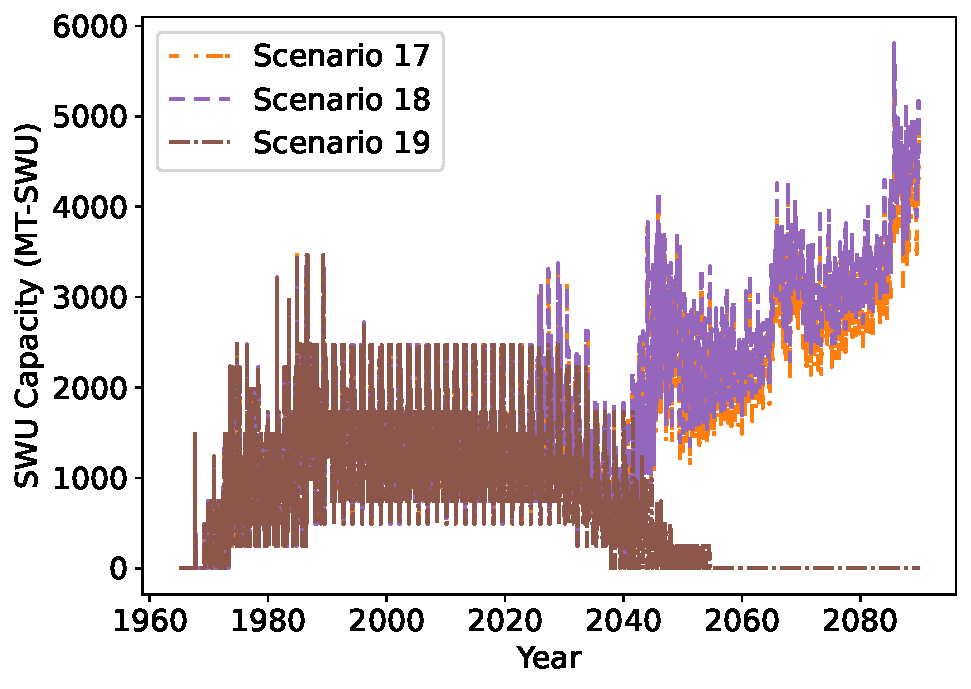
\includegraphics[width=\textwidth]{1percent_recycle_swu.pdf}
        \caption{Monthly SWU capacity to support all reactors between 2025-2090.}
        \label{fig:1percent_recycle_swu_all}
    \end{subfigure}
    \hfill
    \begin{subfigure}[b]{0.45\textwidth}
        \centering
        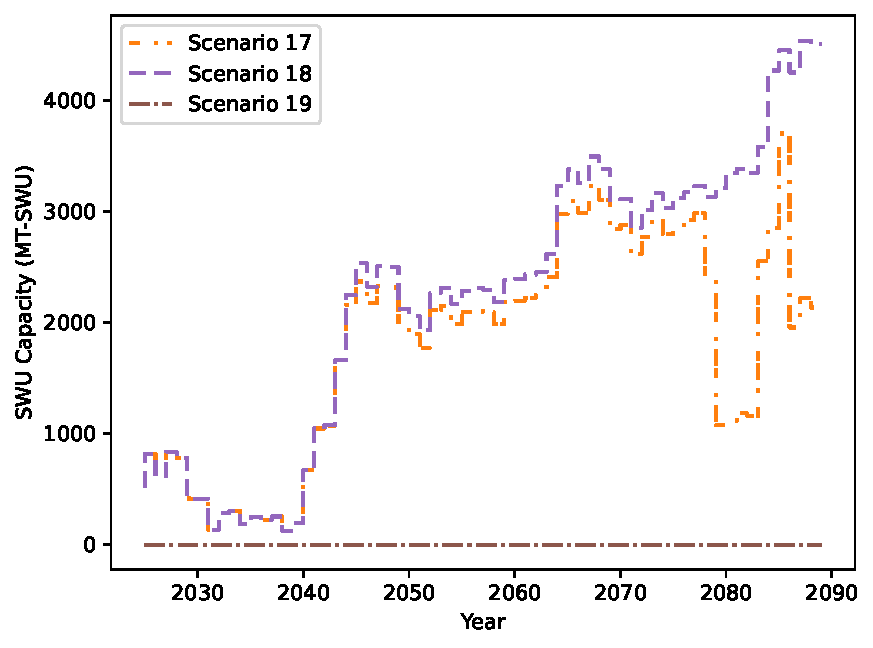
\includegraphics[width=\textwidth]{1percent_recycle_AR_swu.pdf}
        \caption{Annual average SWU capacity to support 
        advanced reactors between 2025-2090.}
        \label{fig:1percent_recycle_swu_AR}
    \end{subfigure}
       \caption{\gls{SWU} capacity required to support reactors in Scenarios 14-16.}
       \label{fig:1percent_recycle_swu}
\end{figure}

Table \ref{tab:s17-19_swu} reports the metrics for the \gls{SWU} capacities 
required in Scenarios 17-19. Scenarios 17 and 18 require less 
\gls{SWU} capacity than Scenario 13, because the use of 
reprocessing and plutonium-based fuel decreases the need for 
enriched uranium. Scenarios 17 and 18 require more \gls{SWU} 
capacity than Scenarios 9 and 12, because of the difference in 
the advanced reactors deployed between these scenarios. These results 
vary from the results of the no growth scenarios, in which the 
average \gls{SWU} of the closed fuel cycles were smaller than the 
average capacity in the once-through fuel cycles. This difference 
between the energy demand curves is a result of the deployment 
scheme artificially inflating the number of \glspl{MMR} built. This 
extra deployment of \glspl{MMR} in the 1\% growth scenarios that 
deploy the \gls{MMR} increases the \gls{SWU} capacity because the 
\gls{MMR} requires more enriched uranium and a higher enrichment 
level than the Xe-100 and VOYGR. Therefore, the deployment scheme 
of the reactors affects the metrics of the transition when changing 
the energy demand. 

\begin{table}[h!]
    \centering 
    \caption{Metrics for \gls{SWU} capacity required to produce 
    enriched uranium in Scenarios 17-19.}
    \label{tab:s17-19_swu}
    \begin{tabular}{c c c c}
        \hline 
        Scenario & Average (MT-SWU/month) & HALEU Average (MT-SWU/month)
         & Maximum (MT-SWU) \\
        \hline 
        17 & 2,049 & 2,009 & 5,504 \\
        18 & 2,207 & 2,168 & 5,806 \\
        19 & 0 & 0 & 0 \\
        \hline
        
    \end{tabular}
\end{table}

\section{Separated actinide mass}
The next metric of interest is the separated actinide mass sent 
from the separations facility to the fuel fabrication facility. 
The separated actinide masses include any actinides separated 
from \gls{SNF} (i.e., uranium, neptunium, plutonium, and 
americium). 
This metric provides context on how much material is available for 
producing plutonium-based fuels, and has implications on 
separations and fabrication facility size needs. Separations facilities 
are deployed starting in 2020, so these results begin in 2020 instead 
of 2025 like the other results. 

\subsection{No growth scenarios}
Figure \ref{fig:nogrowth_recycle_sep_pu} shows the separated plutonium 
masses in Scenarios 14-16. Scenario 16 has the most separated 
plutonium of the three scenarios, which is consistent with the other 
results of these scenarios. Scenarios 14 and 15 have very little 
separated plutonium compared with Scenario 16. The primary reason 
for this large difference is the elements separated out in 
each scenario. In Scenario 16, four different actinide elements 
are separated out from the fission products (uranium, neptunium,
plutonium, and americium), but in Scenarios 14 and 15 only plutonium 
is separated out. The inclusion of other elements to separate out 
in Scenario 16 (primarily the uranium, which consists of up to 
93\% of \gls{SNF}), increases the mass of material  
separated out from the \gls{SNF}. 

\begin{figure}[h!]
    \centering
    \begin{subfigure}[b]{0.49\textwidth}
        \centering
        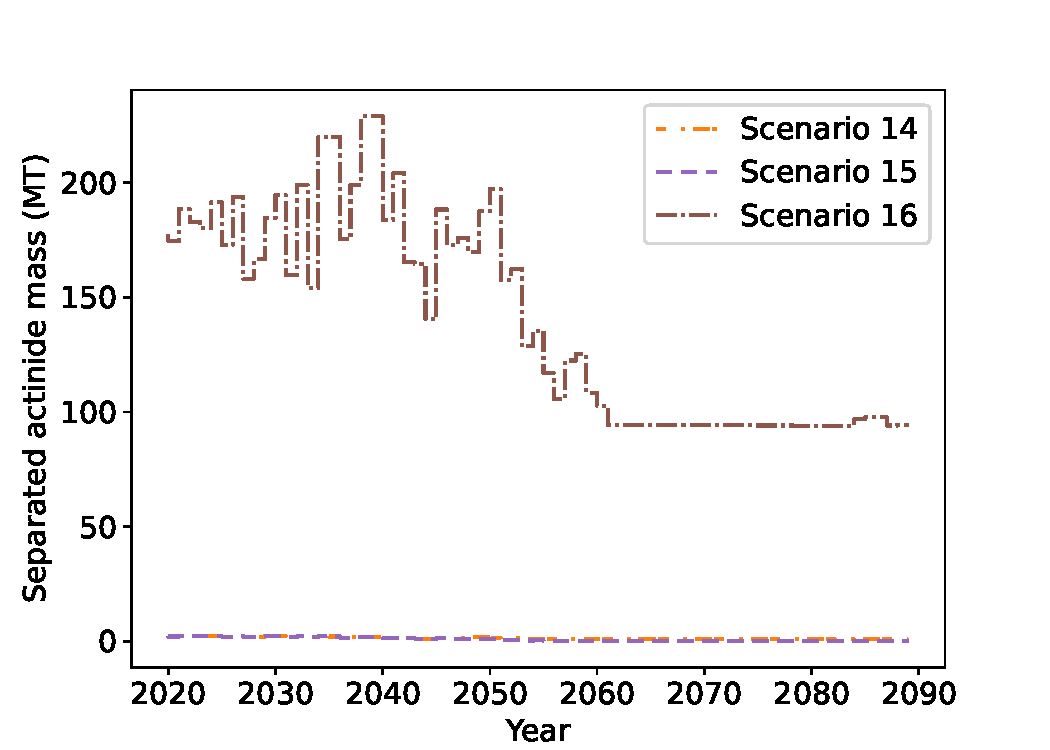
\includegraphics[width=\textwidth]{nogrowth_recycle_sep_pu.pdf}
        \caption{Monthly mass between 2020-2090.}
        \label{fig:nogrowth_recycle_sep_pu_all}
    \end{subfigure}
    \hfill
    \begin{subfigure}[b]{0.49\textwidth}
        \centering
        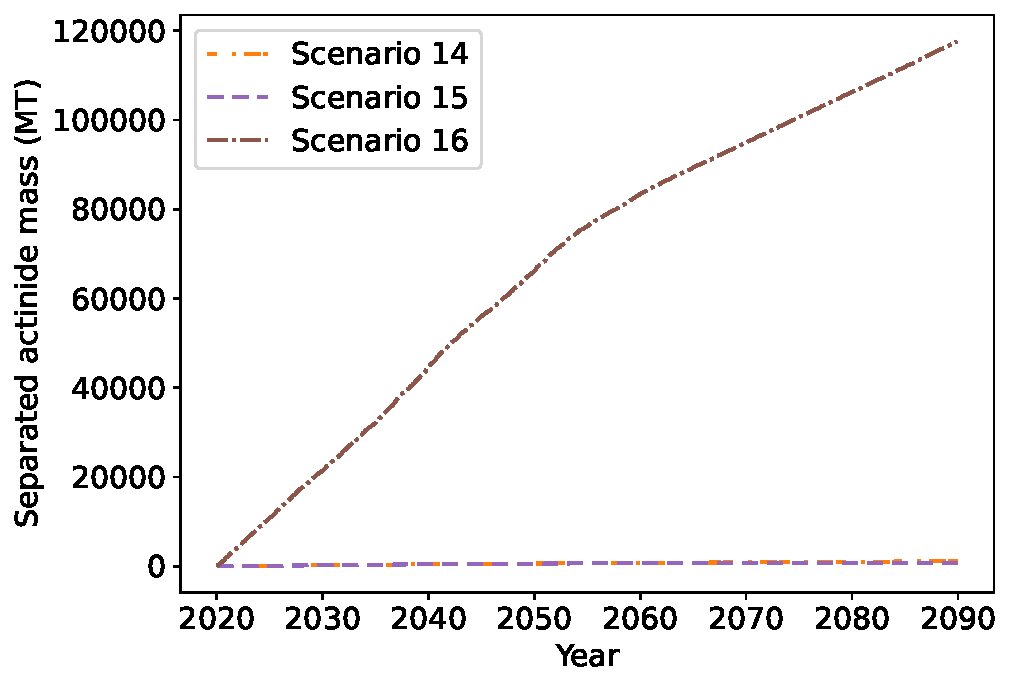
\includegraphics[width=\textwidth]{nogrowth_recycle_sep_pu_cumulative.pdf}
        \caption{Cumulative mass between 2020-2090.}
        \label{fig:nogrowth_recycle_sep_pu_cumulative}
    \end{subfigure}
       \caption{Mass of separated actinides sent from the 
       separations facility to fuel fabrication in Scenarios 14-16.}
       \label{fig:nogrowth_recycle_sep_pu}
\end{figure}

Table \ref{tab:s14-16_sep_pu} reports the metrics of the separated 
plutonium in Scenarios 14-16. All three scenarios experience a 
maximum amount of separated actinides at the same time, in 
November 2031. This timing corresponds with \gls{SNF} discharged 
from \glspl{LWR} in November 2025 and fuel from advanced reactors
discharged in October 2031. This consistency in the maximum 
for these three scenarios emphasizes the importance of reprocessing 
the \gls{SNF} from \glspl{LWR} in these metrics.  

\begin{table}[h!]
    \centering 
    \caption{Metrics of separated actinide masses of between 2020-2090 in 
    Scenarios 14-16.}
    \label{tab:s14-16_sep_pu}
    \begin{tabular}{c c c c}
        \hline 
        Scenario & Average (MT/month) & Maximum (MT) & Cumulative (MT) \\
        \hline
        14 & 1.372 & 4.735 & 1,150\\
        15 & 0.840 & 4.735 & 705.0\\
        16 & 140.1 & 454.3 & 117,584\\
        \hline
    \end{tabular}
\end{table}

From the metrics in Table \ref{tab:s14-16_sep_pu}, the metrics for 
the separated actinide masses in Scenario 16 are two orders of 
magnitude greater than the metrics in Scenarios 14 and 15. The metrics 
for Scenario 16 are also larger than the plutonium-based fuel metrics 
for the scenario in Table \ref{tab:s14-16_mox}. The larger mass 
of separated actinide material than plutonium-based fuels required by 
the reactors drives the lack of enriched uranium to support these 
reactors. The difference between the two material streams stems 
from the reprocessing of uranium from \gls{LWR} fuel, which constitutes 
about 93\% of the \gls{LWR} \gls{SNF}. Therefore, reprocessing 
uranium from \gls{LWR} \gls{SNF} plays an important role in supporting 
this fuel cycle. Between 2060-2090 (after all spent fuel from 
\glspl{LWR} is processed) the \glspl{SFR} require an 
average of 90.3 MT/month of U/TRU fuel, and an average of 95.2 
MT/month of separated actinides. Therefore, the \gls{SFR} could 
still sustain producing enough plutonium-based 
fuel from reprocessing \gls{SFR} \gls{SNF}.

Scenario 16 models the reprocessed uranium as being part of 
the fresh reprocessed fuel. Therefore, it is likely that 
fabricating the reprocessed fuel would not need the natural
uranium masses defined in Table \ref{tab:s14-16_natU}. If this 
production method is possible, then the natural uranium needs 
of the fuel cycle would drop to near-zero, further 
emphasizing how a closed fuel cycle can help minimize
natural uranium needs. 

\subsection{1\% growth scenarios}
Figure \ref{fig:1percent_recycle_sep_pu} shows the mass of separated 
actinide material in Scenarios 17-19. Similar to the no growth 
scenarios, Scenario 19 has a much greater mass of separated 
actinide material than Scenarios 17 and 18. The greater mass in 
Scenario 19 is a result of multiple actinide elements being 
separated out from the \gls{SNF}, compared with only 
plutonium separated in Scenarios 17 and 18, as well as more fuel 
being reprocessed in Scenario 19. 

\begin{figure}[h!]
    \centering
    \begin{subfigure}[b]{0.49\textwidth}
        \centering
        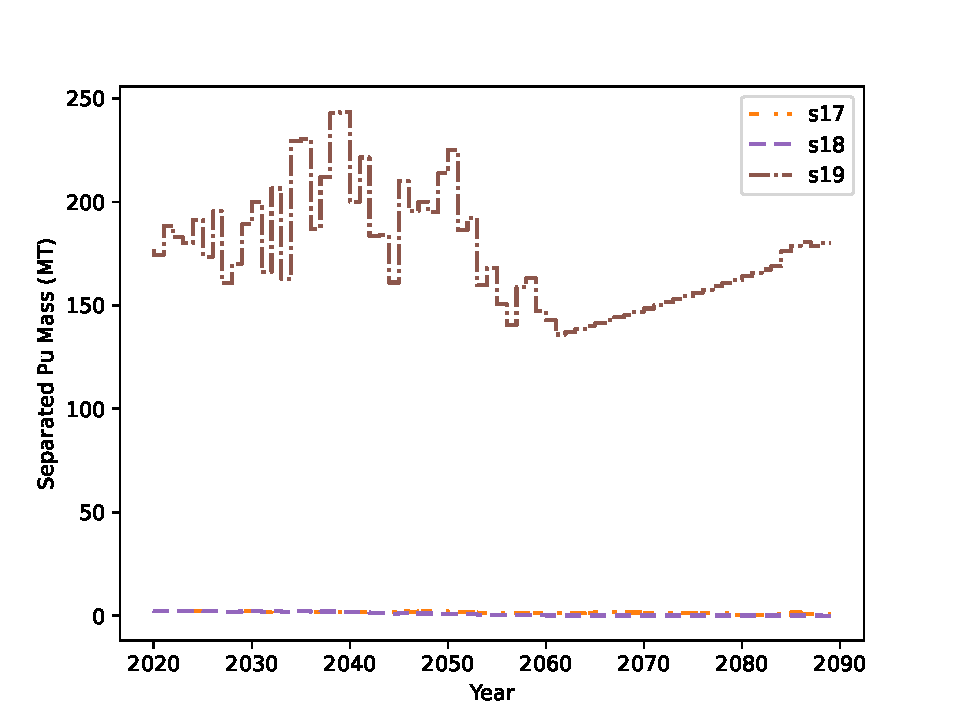
\includegraphics[width=\textwidth]{1percent_recycle_sep_pu.pdf}
        \caption{Mass 
        at each time step between 2020-2090.}
        \label{fig:1percent_recycle_sep_pu_all}
    \end{subfigure}
    \hfill
    \begin{subfigure}[b]{0.49\textwidth}
        \centering
        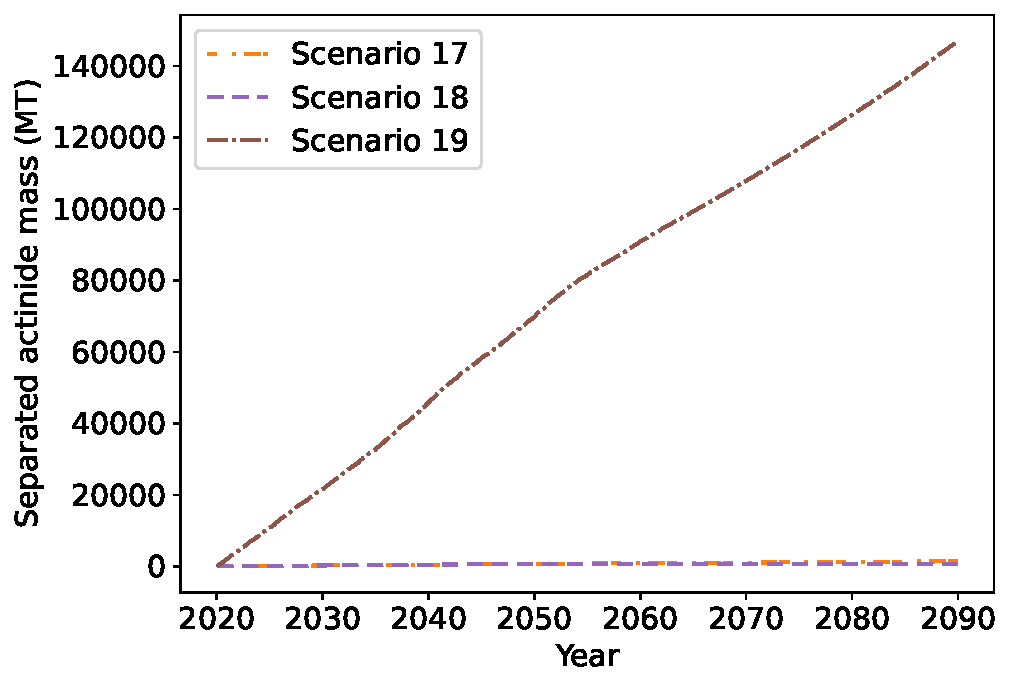
\includegraphics[width=\textwidth]{1percent_recycle_sep_pu_cumulative.pdf}
        \caption{Cumulative mass 
        at each time step between 2020-2090.}
        \label{fig:1percent_recycle_sep_pu_cumulative}
    \end{subfigure}
       \caption{Separated plutonium masses in Scenarios 17-19.}
       \label{fig:1percent_recycle_sep_pu}
\end{figure}

Table \ref{tab:s17-19_sep_pu} reports the metrics of the separated 
actinide masses on Scenarios 17-19. Scenarios 17 and 18 have the 
maximum separated plutonium mass in November 2031, the same time 
as the maximum in Scenarios 14 and 15. The consistency in the 
maximum separated actinide mass in all four of the limited 
recycle scenarios emphasizes the importance of reprocessing the 
\gls{LWR} \gls{SNF} in these scenarios. 

\begin{table}[h!]
    \centering 
    \caption{Mass of separated plutonium between 2020-2090 in Scenarios 
    17-19.}
    \label{tab:s17-19_sep_pu}
    \begin{tabular}{c c c c}
        \hline 
        Scenario & Average (MT/month) & Maximum (MT) & Cumulative (MT) \\
        \hline
        17 & 1.715 & 4.735 & 1,439\\
        18 & 0.854 & 4.735 & 716.4\\
        19 & 175.0 & 500.0 & 146,837\\
        \hline
    \end{tabular}
\end{table}

Figure 
\ref{fig:recycle_sep_pu} shows the annual average and cumulative 
separated actinide mass in Scenarios 14, 15, 17, and 18. All four of 
these scenarios have the same separated actinide masses until 
November 2028, Scenarios 14 and 15 have the same separated actinide 
mass until November 2041, and Scenarios 17 and 18 have the same separated 
actinide mass until February 2042. The similarities between these four 
scenarios is a result of the \gls{LWR} \gls{SNF} driving the amount 
of available separated actinide material, and the use of the 
same advanced reactor build share for scenarios of the same growth. 
However, the fuel considered for reprocessing has a greater impact 
on the amount of separated actinide material available than the 
energy demand. Scenarios 15 and 18 differ by a maximum of 41 kg of 
separated actinide material for a single time step, while Scenarios 
14 and 17 differ by a maximum of 1.4 MT in a single time step. 

\begin{figure}[h!]
    \centering
    \begin{subfigure}[b]{0.49\textwidth}
        \centering
        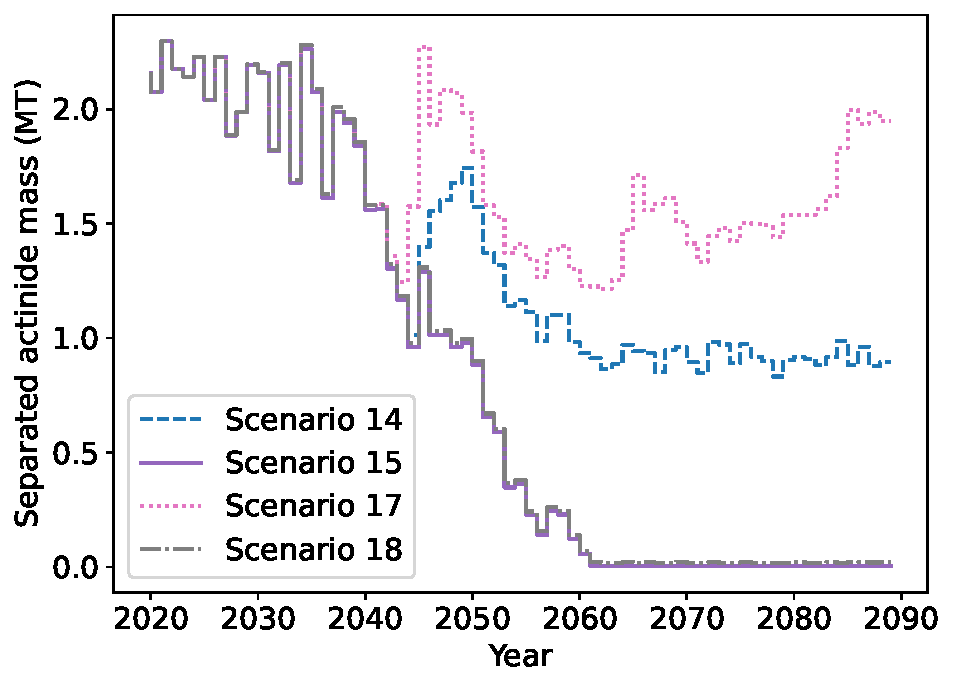
\includegraphics[width=\textwidth]{sep_pu_compare.pdf}
        \caption{Annual average between 2020-2090.}
        \label{fig:_recycle_sep_pu_all}
    \end{subfigure}
    \hfill
    \begin{subfigure}[b]{0.49\textwidth}
        \centering
        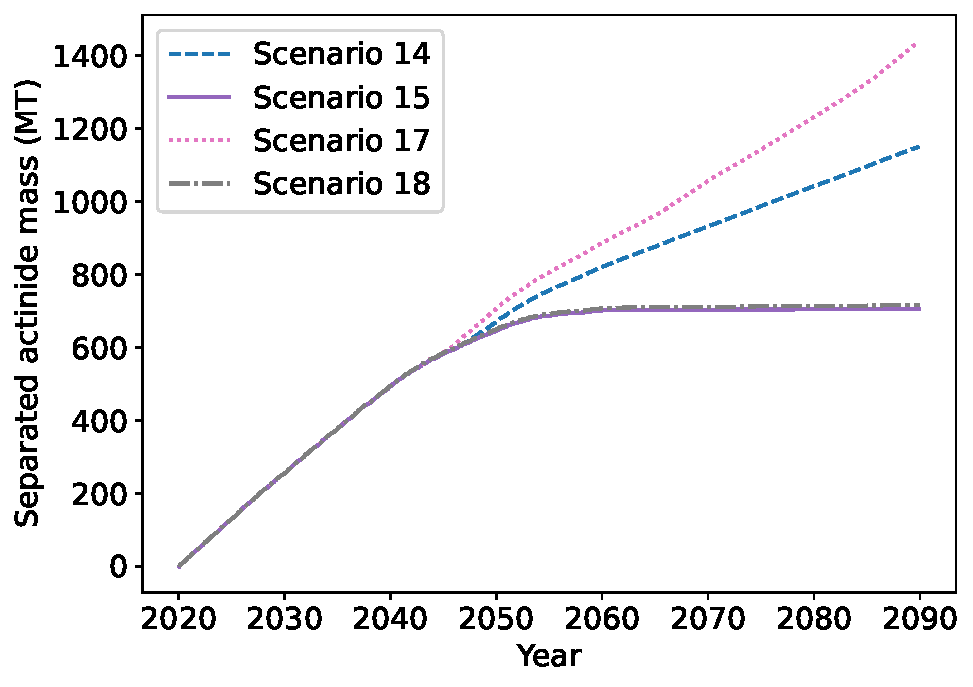
\includegraphics[width=\textwidth]{sep_pu_compare_cumulative.pdf}
        \caption{Cumulative mass between 2020-2090.}
        \label{fig:recycle_sep_pu_cumulative}
    \end{subfigure}
       \caption{Separated plutonium masses in the limited 
       recycle fuel cycles, Scenarios 14, 15, 17,18.}
       \label{fig:recycle_sep_pu}
\end{figure}

\section{Spent nuclear fuel and high level waste}
This section provides the results of the \gls{SNF} and \gls{HLW} sent 
to disposal in the closed fuel cycles. The once-through scenario 
results only defined the \gls{SNF} sent for disposal because all 
of the materials needing disposal in those scenarios are \gls{SNF}. 
With the addition of the separation step, the \gls{SNF} discharged 
from reactors gets separated into two different material streams, 
one of the separated plutonium and one of \gls{HLW} that is sent 
for disposal. \gls{SNF} 
is the spent fuel from each of the reactors that is disposed 
with reprocessing. \gls{HLW} is 
the waste (e.g., fission products) separated out from the 
reprocessed \gls{SNF}. 

\subsection{No growth scenarios}
This section presents the results of the \gls{SNF} and 
\gls{HLW} masses that are sent for disposal in a 
material sink in the no growth recycle scenarios. 

\subsubsection{Spent nuclear fuel}
Figure \ref{fig:nogrowth_recycle_snf} shows the 
masses of advanced reactor \gls{SNF} disposed of 
in Scenarios 14-16. In Scenario 14 only the spent \gls{MOX} 
fuel is disposed of, in Scenario 15 the spent \gls{MOX} as 
well as the spent \gls{MMR} and Xe-100 fuels are disposed of, 
and no \gls{SNF} is disposed of in Scenario 16. The disposal of 
\gls{MMR} \gls{SNF} in Scenario 15 leads to the single times 
with larger disposal masses, because of the single-batch 
fueling scheme of the \gls{MMR}. The additional fuel that 
is disposed of in Scenario 15, compared with Scenarios 
14 and 16, increases the amount of \gls{SNF} disposed. 

\begin{figure}[h!]
    \centering
    \begin{subfigure}[b]{0.49\textwidth}
        \centering
        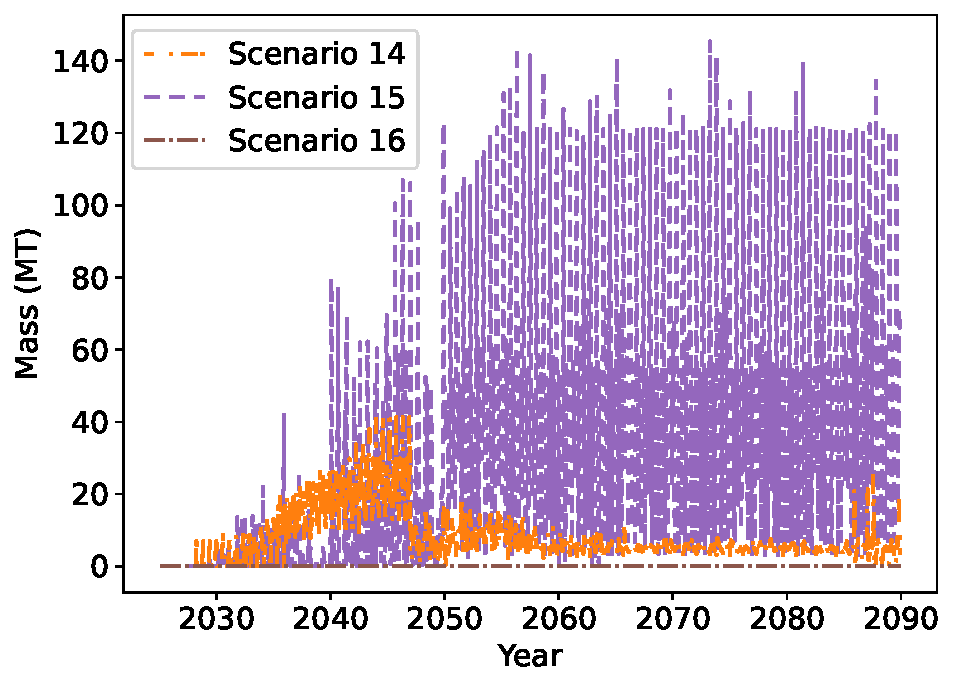
\includegraphics[width=\textwidth]{nogrowth_recycle_snf.pdf}
        \caption{Monthly mass sent for disposal 
        at each time step between 2025-2090.}
        \label{fig:nogrowth_recycle_snf_all}
    \end{subfigure}
    \hfill
    \begin{subfigure}[b]{0.49\textwidth}
        \centering
        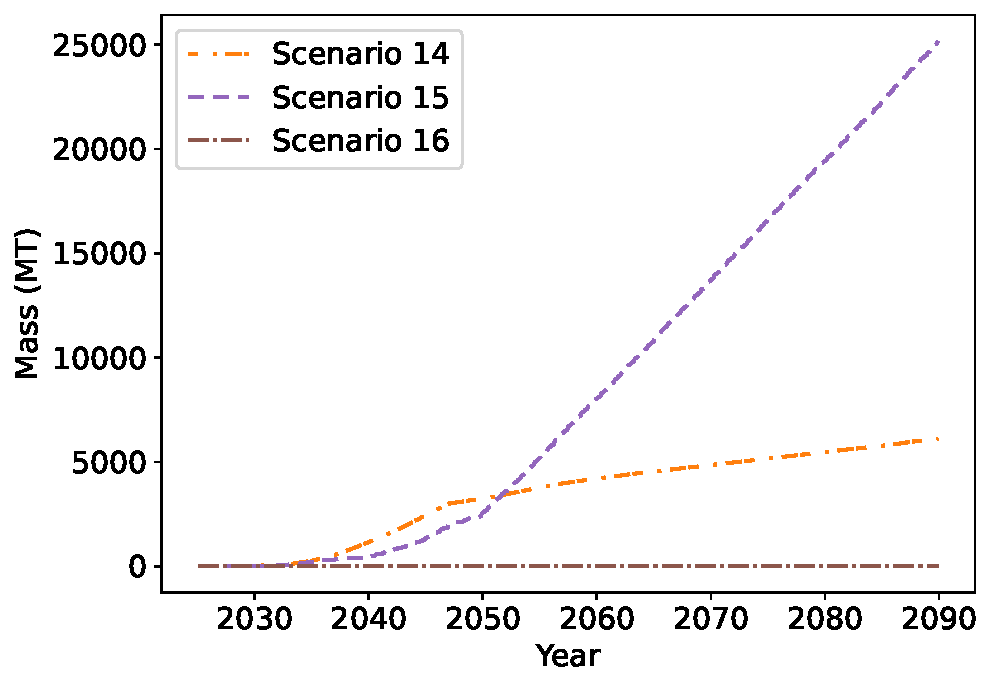
\includegraphics[width=\textwidth]{nogrowth_recycle_snf_cumulative.pdf}
        \caption{Cumulative mass sent for disposal 
        at each time step between 2025-2090.}
        \label{fig:nogrowth_recycle_snf_cumulative}
    \end{subfigure}
       \caption{Spent nuclear fuel disposed of in Scenarios 14-16.}
       \label{fig:nogrowth_recycle_snf}
\end{figure}

Table \ref{tab:s14-16_snf} reports the metrics for the \gls{SNF} disposal 
in Scenarios 14-16. The values in this table are smaller than 
the \gls{SNF} masses in the once-through scenarios (Table 
\ref{tab:nogrowth_waste}). This decrease in \gls{SNF} disposal is 
a result of the reprocessing in Scenarios 14-16, and is an 
advantage of a closed fuel cycle. 

\begin{table}[h!]
    \centering 
    \caption{Mass of SNF disposed of between 2025-2090 in 
    Scenarios 14-16.}
    \label{tab:s14-16_snf}
    \begin{tabular}{c c c c}
        \hline 
        Scenario & Average (MT/month) & Maximum (MT) & Cumulative (MT) \\
        \hline
        14 & 7.835 & 41.33 & 6,103\\
        15 & 32.29 & 145.4 & 25,153 \\
        16 & 0 & 0 & 0 \\
        \hline
    \end{tabular}
\end{table}

Based on these values and the results in 
Figure \ref{fig:nogrowth_recycle_snf}, including more fuel for 
reprocessing can greatly reduce the mass of \gls{SNF}. All three of 
these scenarios have a cumulative \gls{SNF} mass smaller than 
that of all of the once-through scenarios. Additionally, 
the \gls{SNF} from advanced reactors in all three of these scenarios 
is less than the 70,000 MT limit for Yucca Mountain. The reduction in 
\gls{SNF} mass compared with the once-through scenarios highlights 
an advantage of closed fuel cycles. 

\subsubsection{High level waste}
Figure \ref{fig:nogrowth_recycle_hlw} shows the 
\gls{HLW} masses for disposal in Scenarios 14-16. Scenario 
14 results in the most \gls{HLW}, because more 
material is reprocessed in this scenario than in Scenario 15, 
and less actinide material is separated out than in 
Scenario 16. The \gls{HLW} mass in Scenario 15 reaches a 
near-zero level around 2060, because all of the \gls{LWR} 
\gls{SNF} is reprocessed by this time which leaves only
the VOYGR \gls{SNF} available for reprocessing. A 
maximum of 7 VOYGRs are deployed at a time in Scenario 
15, so there is very little \gls{SNF} reprocessed and 
little \gls{HLW} generated after 2060. 

\begin{figure}[h!]
    \centering
    \begin{subfigure}[b]{0.49\textwidth}
        \centering
        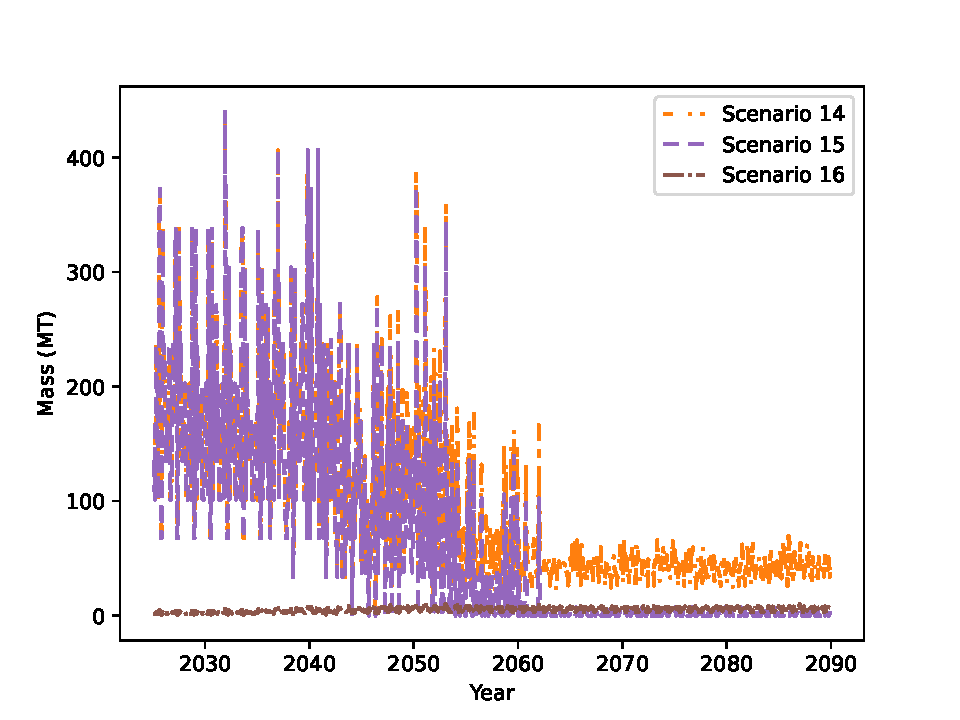
\includegraphics[width=\textwidth]{nogrowth_recycle_hlw.pdf}
        \caption{Monthly mass sent for disposal 
        at each time step between 2025-2090.}
        \label{fig:nogrowth_recycle_hlw_all}
    \end{subfigure}
    \hfill
    \begin{subfigure}[b]{0.49\textwidth}
        \centering
        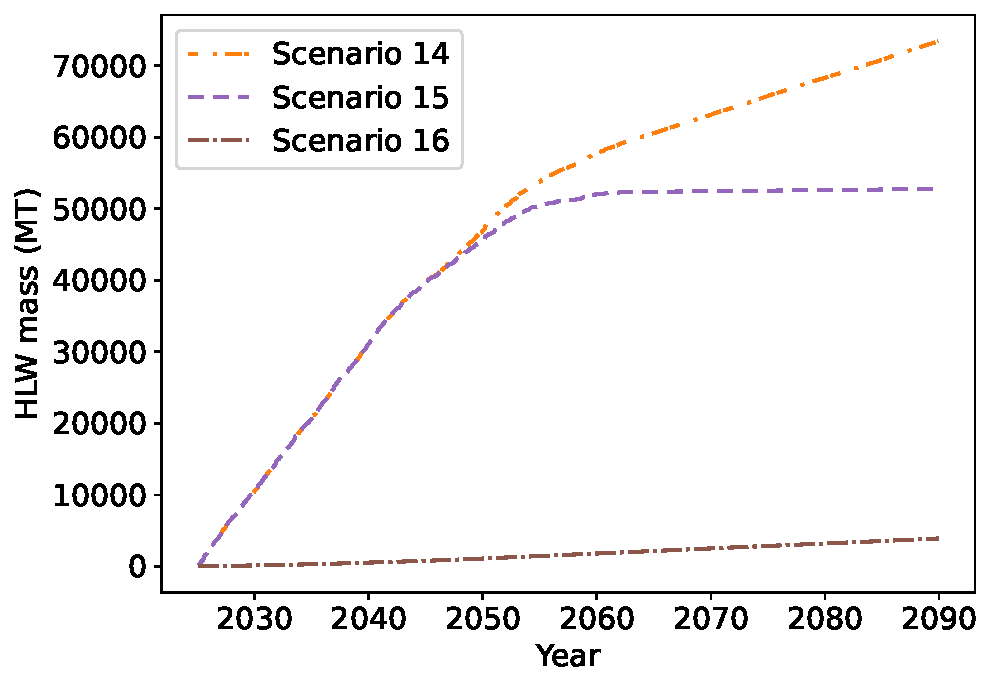
\includegraphics[width=\textwidth]{nogrowth_recycle_hlw_cumulative.pdf}
        \caption{Cumulative mass sent for disposal 
        at each time step between 2025-2090.}
        \label{fig:nogrowth_recycle_hlw_cumulative}
    \end{subfigure}
       \caption{Mass of \gls{HLW} disposed of in Scenarios 14-16.}
       \label{fig:nogrowth_recycle_hlw}
\end{figure}

Table \ref{tab:s14-16_hlw} reports the metrics for the \gls{HLW} 
in Scenarios 14-16. Scenario 16 generates very little 
\gls{HLW} because the actinide material separated out 
comprises most of the mass of the \gls{SNF}. The \gls{HLW} 
masses for Scenarios 14 and 15 are larger than the \gls{SNF} 
masses for these scenarios, and are larger than the \gls{SNF} 
masses of the no growth, once-through scenarios, except 
Scenario 5. The increase 
comes from the inclusion of \gls{LWR} \gls{SNF} for reprocessing 
in these scenarios. Including this \gls{SNF} increases the 
disposed material mass because this metric is not solely focused 
on material from the advanced reactors like it was for 
the once-through scenarios. The average for 
Scenario 14 is similar to the average \gls{SNF} disposed of 
between 2025-2055 in Scenario 1 (94.27 MT/month). 

\begin{table}[h!]
    \centering 
    \caption{Mass of HLW disposed of between 2025-2090 in 
    Scenarios 14-16.}
    \label{tab:s14-16_hlw}
    \begin{tabular}{c c c c}
        \hline 
        Scenario & Average (MT/month) & Maximum (MT) & Cumulative (MT) \\
        \hline
        14 & 94.21 & 440.2 & 73,389\\
        15 & 67.73 & 440.2 & 52,764\\
        16 & 5.011 & 10.09 & 3,903\\
        \hline
    \end{tabular}
\end{table}

The \gls{HLW} in each of these scenarios has a different 
composition than the \gls{SNF}, but both waste streams 
still require a geologic repository for final 
disposal. Therefore, both the \gls{SNF} and \gls{HLW} 
masses must be considered for evaluating repository 
capacities. The \gls{HLW} in Scenario 14 is more than 
the 70,000 MT limit of Yucca Mountain, so a second 
repository would be needed to disposal of both waste 
streams. The \gls{SNF} and \gls{HLW} materials in 
Scenario 15 sum to 77,917 MT, meaning that a second 
repository would be needed to support this scenario 
as well. These material streams sum to 3,903 MT in 
Scenario 16, which means that the Yucca Mountain 
limit of 70,000 MT would be sufficient to support this 
scenario. 


\subsection{1\% growth scenarios}
This section presents the results of the \gls{SNF} and 
\gls{HLW} masses that are sent for disposal in a 
material sink in the 1\% growth recycle scenarios. 

\subsubsection{Spent nuclear fuel}
Figure \ref{fig:nogrowth_recycle_snf} shows the mass of \gls{SNF} 
disposed of in Scenarios 17-19. These results follow a similar 
pattern to the no growth scenarios; Scenario 18 disposes of 
the most \gls{SNF}, followed by Scenario 17, and Scenario 
19 does not have any \gls{SNF} disposed of. This pattern 
emerges because of the material available for reprocessing 
in each scenario. The more \gls{SNF} reprocessed, the less 
\gls{SNF} disposed. 

\begin{figure}[h!]
    \centering
    \begin{subfigure}[b]{0.49\textwidth}
        \centering
        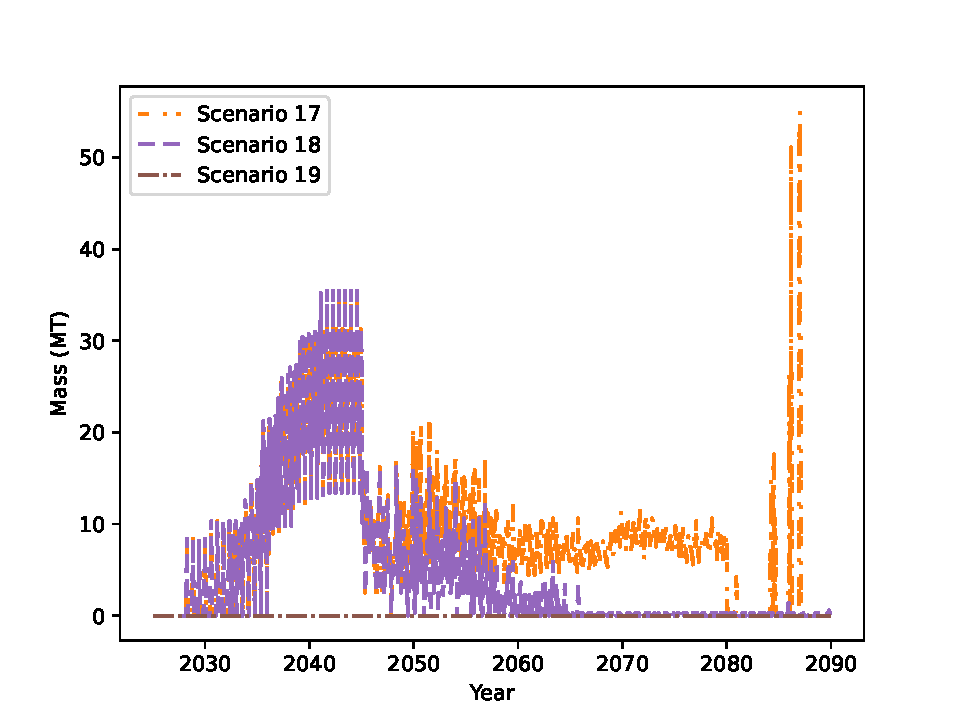
\includegraphics[width=\textwidth]{1percent_recycle_snf.pdf}
        \caption{Monthly mass between 2025-2090.}
        \label{fig:1percent_recycle_snf_all}
    \end{subfigure}
    \hfill
    \begin{subfigure}[b]{0.49\textwidth}
        \centering
        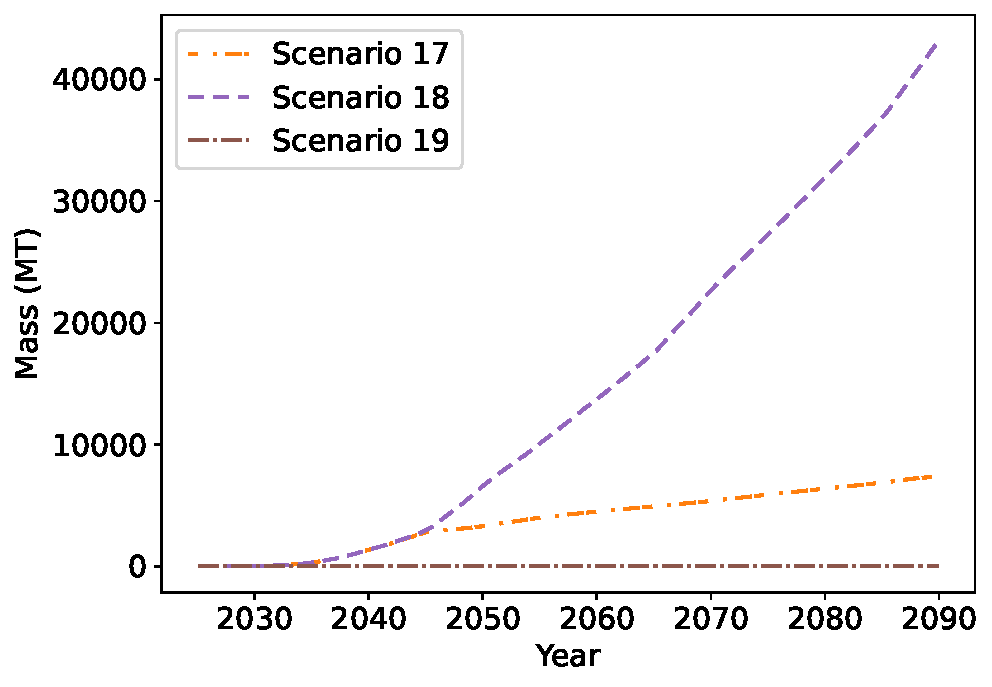
\includegraphics[width=\textwidth]{1percent_recycle_snf_cumulative.pdf}
        \caption{Cumulative mass between 2025-2090.}
        \label{fig:1percent_recycle_snf_cumulative}
    \end{subfigure}
       \caption{Spent nuclear fuel disposed of in Scenarios 17-19.}
       \label{fig:1percent_recycle_snf}
\end{figure}

Table \ref{tab:s17-19_snf} reports the metrics of the \gls{SNF} 
disposed of in Scenarios 17-19. Scenarios 17 and 19 dispose of 
less \gls{SNF} than Scenarios 8-13, but Scenario 18 disposes of 
more \gls{SNF} than Scenario 9. Scenario 9 only deploys the 
Xe-100, while Scenario 18 has an artificially inflated number of 
\glspl{MMR} deployed, and the Xe-100 uses less fuel than the 
\gls{MMR}. We observe this effect in Scenario 18 and not 
Scenario 17, because \gls{MMR} \gls{SNF} is reprocessed in 
Scenario 17 but not in Scenario 18. Therefore the \gls{MMR} 
\gls{SNF} in Scenario 17 get split between the 
\gls{HLW} and plutonium-based fuel material streams. The \gls{SNF} mass comparisons 
between the closed and once-through fuel cycles are consistent 
with the other results: reprocessing fuel reduces material metrics, 
but the reactors deployed are the primary driver of the metrics. 

\begin{table}[h!]
    \centering 
    \caption{Mass of SNF disposed of between 2025-2090 in 
    Scenarios 17-19.}
    \label{tab:s17-19_snf}
    \begin{tabular}{c c c c}
        \hline 
        Scenario & Average (MT/month) & Maximum (MT) & Cumulative (MT) \\
        \hline
        17 & 9.542 & 35.47 & 7,433\\
        18 & 55.34 & 157.4 & 43,113\\
        19 & 0 & 0 & 0 \\
        \hline
    \end{tabular}
\end{table}


\subsubsection{High level waste}
Finally, Figure \ref{fig:1percent_recycle_hlw} shows the \gls{HLW} 
mass disposed of in Scenarios 17-19. These results are similar to 
the results from the no growth closed fuel cycle scenarios; Scenario 
17 has the most \gls{HLW} mass, followed by Scenario 18, and Scenario 
19. 
\begin{figure}[h!]
    \centering
    \begin{subfigure}[b]{0.49\textwidth}
        \centering
        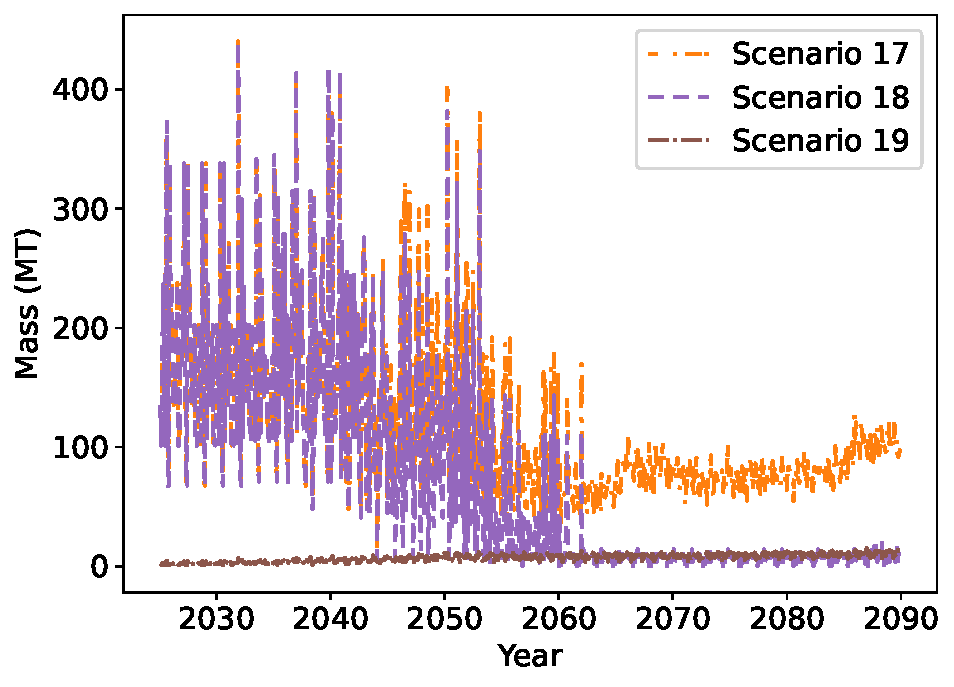
\includegraphics[width=\textwidth]{1percent_recycle_hlw.pdf}
        \caption{Monthly mass of HLW sent for disposal 
        at each time step between 2025-2090.}
        \label{fig:1percent_recycle_hlw_all}
    \end{subfigure}
    \hfill
    \begin{subfigure}[b]{0.49\textwidth}
        \centering
        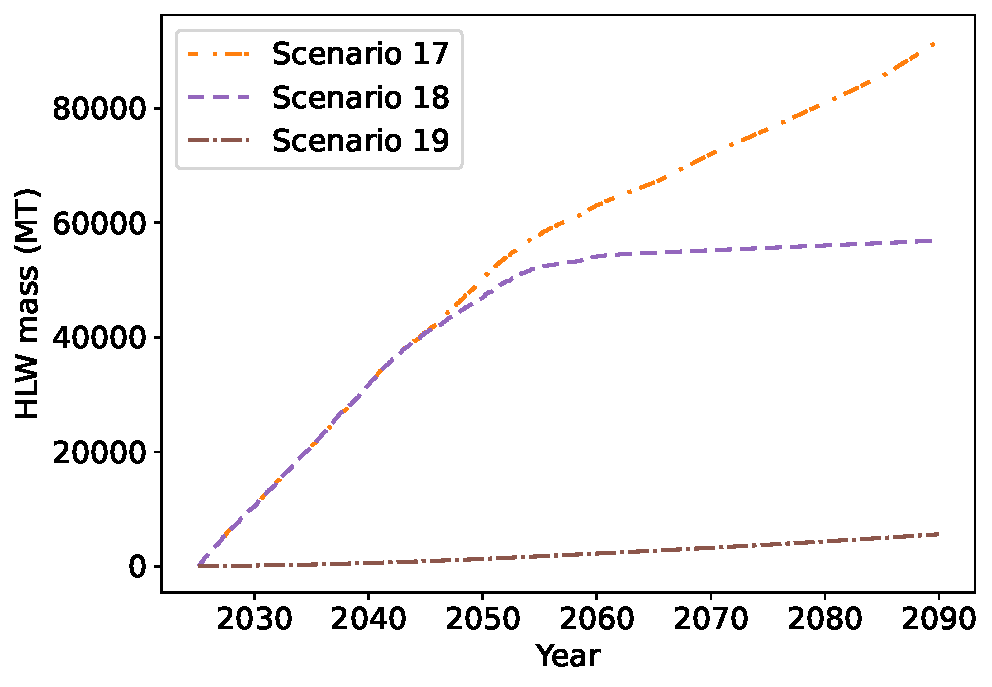
\includegraphics[width=\textwidth]{1percent_recycle_hlw_cumulative.pdf}
        \caption{Cumulative mass of HLW sent for disposal 
        at each time step between 2025-2090.}
        \label{fig:1percent_recycle_hlw_cumulative}
    \end{subfigure}
       \caption{\gls{HLW} disposed of in Scenarios 17-19.}
       \label{fig:1percent_recycle_hlw}
\end{figure}

Table \ref{tab:s17-19_hlw} reports the metrics for the \gls{HLW} mass 
in Scenarios 17-19. These values are almost all larger than the 
values for the no growth fuel cycles (Table \ref{tab:s14-16_hlw}), but 
Scenarios 17 and 18 have the same maximum value as Scenarios 14 and 15. The 
consistency in the maximum value in these four scenarios corresponds to 
\gls{LWR} \gls{SNF} reprocessing, and emphasizes the impact that 
\gls{LWR} \gls{SNF} has on the material availability and requirements 
of these fuel cycles. 

\begin{table}[h!]
    \centering 
    \caption{Mass of HLW disposed of between 2025-2090 in 
    Scenarios 17-19.}
    \label{tab:s17-19_hlw}
    \begin{tabular}{c c c c}
        \hline 
        Scenario & Average (MT/month) & Maximum (MT) & Cumulative (MT) \\
        \hline
        17 & 117.7 & 440.2 & 91,670 \\
        18 & 73.06 & 440.2 & 56,915 \\
        19 & 7.195 & 15.29 & 5,604 \\
        \hline
    \end{tabular}
\end{table}

The cumulative \gls{HLW} mass in Scenario 17 is larger than the 70,000
MT limit for Yucca Mountain. The cumulative \gls{HLW} mass 
in Scenario 18 is less than the 70,000 MT limit, but combining this with 
the 43,113 MT of \gls{SNF} pushes the total waste over the 70,000 MT 
limit. Therefore, a second repository would be needed to support 
material disposal in these scenarios. The total \gls{HLW} and \gls{SNF} 
masses in Scenario 19 are less than the 70,000 MT limit, which means 
that the one repository would be sufficient to support the disposal 
needs of this scenario. 